% Chapter 

\chapter{\color{thesisBlue} Using Generative Models of Natural Images to Define Neural Tuning Manifolds} % Main chapter title

\label{ch:maps} % For referencing the chapter elsewhere, use \ref{ch:maps} 

%----------------------------------------------------------------------------------------

% Define some commands to keep the formatting separated from the content 
%\newcommand{\keyword}[1]{\textbf{#1}}

%------------------------------------------------------------------------------------


%Investigations into sensory coding in the visual system have typically relied on the use of either simple, unnatural visual stimuli, or natural images. Simple stimuli, such as gabors, have been effective when looking at single neurons in early visual areas such as V1, but seldom produce large responses from mid-level visual neurons or neural populations with diverse tuning. Many types of ``Naturalistic" image models have been developed recently which bridge the gap between overly-simple stimuli and experimentally infeasible natural images. These stimuli can vary along a large number of feature dimensions, introducing new challenges when trying to map those features to neural activity. We propose a method that searches high-dimensional stimulus spaces for neural tuning in a closed-loop experimental design. Stimuli are generated in each block by using neural responses to previous stimuli to make predictions about the relationship between the stimulus space and neural response space. We found that these variables contained stronger linear relationships with neural activity than many other forms of image processing, including fourier decomposition or image compression in pixel space.


\section{Introduction}
Research into sensory coding in the visual system focuses on determining what visual features neuronal activity covaries with, i.e. what information is it encoding. Traditional experiments looked at neural responses to simple stimuli such as small patches of light or oriented bars \parencite{Hubel1959}. These hallmark studies uncovered the simple/complex models of V1 neurons, which describe the way in which neurons encode feature information in meaningful ways. \cite{Johnson2008} for example, found that V1 neurons span the range of feature tuning from purely-color to purely-luminance tuned for orientation, while \cite{Garg2019} demonstrated that they are spatially organized by tuning. These luminance and color patches at an orientation are thereby thought to be a visual representation of a neuron receptive field. The closer a stimulus matches a neurons preference, the higher the neuron responds. These stimuli are effective at driving neurons in early visual areas due to the precise arrangement of their inputs. Later in the visual hierarchy, such as V4, it becomes much more difficult to infer the exact tuning properties of neural inputs, and how they combine to form emergent tuning of these neurons. Neurons in area V4 only weakly respond to such stimuli as gabors, as they prefer complex combinations of many features such as contrast, color, orientation, curvature, etc \parencite{Sani2013,Tanigawa2010, Nandy2016}. It is not feasible to systematically test every combination of visual features to accurately describe feature tuning in such brain regions. Here we describe a method for efficiently exploring rich stimulus spaces to find relationships between sensory features and neural responses.

In these experiments, we used a \gls{gan} as our high-dimensional feature space. A \gls{gan} is a type of artificial neural network trained to represent the high-order statistics from a training set of data using a lower-dimensional set of `latent’ variables. In a \gls{gan} trained on faces for example, one of these variables may be the age of the person \parencite{Karras2019}. The complex combinations of visual features that makes someone look older or younger can be summarized with a one-dimensional variable, and \glspl{gan} can capture that. We sought to investigate if neurons in visual areas V1 and V4 are tuned to the image statistics captured by such a latent variable model. We might expect V4 neurons to be better described by a \gls{gan} model than V1, due to the complexity of feature combinations. Alternatively, the \gls{gan} may be perfectly capable of generating stimuli that accurately describe V1 too, but the linearity or dimensionality of embedding changes. In order to effectively quantify neural tuning in such large stimulus spaces, an efficient search method is required. To this end, we utilized two methods to efficiently explore parts of the GANs latent space that are most likely to result in large neural responses from the population, \gls{pso} and genetic algorithms. 

While the idea of optimizing stimuli for neurons is not new, most of these studies focus on maximizing the response of single neurons \parencite{Ponce2019, Bashivan2019}.  It is unlikely that a single unique stimulus exists such that it maximally excites a diverse neural population. This is especially true in areas like V4, where neurons have complex tuning across many modalities \parencite{Pasupathy2002}. In fact, there are likely many unique stimuli that drive the neural population at similar levels due to contributions from different neurons. To contend with this difficulty, we use two distinct optimization approaches both utilizing the $L^2$ norm of the population response vector. Cowley et al (2017) demonstrated that optimizing for the $L^2$ norm results in a reasonable estimation of the response manifold \parencite{Cowley2017}.

We found several strong relationships (linear and nonlinear) between the latent space of our \gls{gan} and neural activity in both V1 and V4. These relationships arose even when random stimuli were shown, but they were systematically stronger when stimuli were optimized using either \gls{pso} or genetic algorithms. By directly comparing the stimulus embeddings within session and brain area, we found that V1 is consistently more linearly-related to stimulus parameters than V4. This holds true across both \gls{gan} latents and the actual pixel values, indicating that the linearity in neural responses is not a unique feature of the latent space but of processing in the brain. We show here that stimulus tuning in visual neurons can be elucidated using a single experiment, removing the need for assumptions about stimulus parameters, brain region differences, and optimization approaches. The flexibility afforded by this single-experiment approach for describing neuron preferences is a powerful tool for future studies of neural tuning.


\section{Methods}

This project is separated into two adult male rhesus macaques \textit{(Macacca Mulatta)}, one anesthetized experiment and another alert experiment. The stimulus space (\gls{gan}), optimization algorithms, and experimental design (series of static images) were held constant across experiments, but recording methodologies differed. The anesthetized experiment used neuropixels and spikeGLX to record neurons, while the alert experiment used an implanted chronic matrix electrode array with Trellis (Ripple Neuro, TX). 

\subsection*{Anesthetized Experiment}
The subject used in this study was one adult male rhesus macaque \textit{(Macacca Mulatta)}, Tw. All surgical and experimental procedures were performed in accordance with the National Institutes of Health \textit{Guide for the Care and Use of Laboratory Animals} and were approved by the University of Rochester Committee for Animal Research.

\subsubsection*{Surgical Procedures.}
TW was given an initial dose of ketamine (10mg/kg, IM) to induce anesthesia, as well as Atropine (0.05mg/kg, IM) and dexmaethasone (1-4ml/kg, IM). The animal was then maintained on fentanyl (10–25micrograms/kg/h, i.v.), isoflurane ($0.25-1.5\%$), and nitrous oxide (1:2, in oxygen) throughout the experiment. The animal was placed in a steriotaxic frame and body temperature was maintained with a thermostatically controlled heating blanket. The animal was monitored for ECG, temperature, expired $CO_2$, $SPO_2$, and blood pressure to maintain the anesthetic plane. The animal was also given lactated Ringer's with dextrose ($5-20$ml/kg/h, IV) to prevent dehydration, cefazolin (11mg/kg/h, IV) antibiotic. The scalp was first incised and retracted to uncover the right hemisphere from V1 to V4. Craniotomies were made over V1 and V4 in the right hemisphere. The dura was reflected and then the craniotomies filled with agar ($1\%$ in sterile saline). the animal was then fit with contact lenses and paralyzed with vencuronium bromide (0.1-0.6mg/kg/h, IV) before recording. After neurophysiological recordings were complete at 100 hours post initial anesthesia, the animal was euthanized by an injection of sodium pentobarbital (80mg/kg, IV).

\subsubsection*{Neural Recordings.}
Neurophysiological recordings were done using stereotactic implantation of Phase 3B neuropixels \parencite{Jun2017} and recorded using SpikeGLX. Neuropixels were lowered normal to the surface of the cortex in V4 and allowed to baseline for around 30 minutes prior to recording. Following several sessions in V4, we recorded from V1 following the same procedures. Receptive fields were mapped by hand on a whiteboard and listening for spikes. Stimuli were then sized to best cover the conglomerate receptive fields of simultaneously recorded neurons.

\subsubsection*{Visual Stimuli.}
Naturalistic full-color images (as described in methods section: \hyperref[{methods:gan}]{Generative Adversarial Network}) were displayed on a gamma-calibrated 100Hz CRT monitor (ViewSonic, Brea, CA) placed 50-60cm from the animals' eyes. Stimulus control was done with ViSaGe system (Cambridge Research Systems, Rochester, UK) using crs 24-bit color mode in coordination with custom-written Matlab (Mathworks, Natick, MA; for optimization and display) and Python (GAN image generation) routines. Images were displayed on a grey background for 500ms with 1000ms inter-stimulus-intervals. 

\subsubsection*{Data Preprocessing: Anesthetized.}
Spiking data was first run through Kilosort \parencite{Steinmetz2021} to extract individual neurons across channels. Neuron quality was then manually evaluated using Phy before being converted to NeuroData without borders prior to further analyses. Neurons were included for analysis if they were identified as clean, independent units by Kilosort, totaling 1084 neurons in V1 from three optimization experiments (PSO, genetic, random) and 588 neurons in V4 from three separate optimization experiments. 


\subsection*{Alert Experiment}

\subsubsection*{Surgical Procedures}
Prior to any electrical recordings, the subject (Ro) was first implanted with a titanium head holder, trained on behavioral tasks, and then implanted with chronic electrode arrays. All surgeries we performed with isoflurane anesthesia, aseptic technique, and perioperative opiate analgesics in accordance with the National Institutes of Health \textit{Guide for the Care and Use of Laboratory Animals} and were approved by the University of Rochester Committee for Animal Research.

\subsubsection*{Head Holder Implantation} The subject was initially sedated with a 10mg/kg intramuscular injection of ketamine and administered with 0.25mg/kg midazolam, 0.011mg/kg glycopyrrolate, 25mg/kg cefazolin, and 0.2mg/kg meloxicam, all intramuscular. Once anesthetized, we intubated the animal with an endotrachial tube, shaved the animals head, inserted a catheter in the small saphenous vein for infusion of lactated Ringer's solution, then positioned the head in a stereotaxic frame. The anesthesia was maintained with 1.5\% isoflourane throughout the surgery. The surgical site was then thoroughly scrubbed with povidone iodine solution in the preparation of the sterile field. We made a horseshoe-shaped incision (6cm wide by 10cm anterior-posterior) using a \#10 scalpel blade starting from the right brow, cutting caudally parallel to the midline, and ending at the left brow. We then used bone curettes to retract the tissue and clear a large enough surface of skull for the head holder. Sterile gauze soaked in saline was used to keep the tissue moist throughout the surgery. The prefabricated titanium head holder (custum design machined by the university of Pittsburgh cite mat?) attaches to the skull using 16 6mm titanium screws (Veterinary Orthopedic Implants, Saint Augustine, FL) that go through 6 flange straps radially extending from the center of its base. We next bent the straps of the head holder so it fit tightly on the skull. We marked with pencil the final position of the head holder on the skull and made two small incisions in an x through the retracted tissue where the head holder would protrude. We then pushed the exterior portion of the head holder through the dermostomy in the retracted tissue and repositioned it back on the skull. We used a 2mm surgical drillbit and a custum drill stop set to the thickness of the skull to drill through the skull, starting with the lateral-most location of the head holder. Skrews were implanted one a time, alterniting across the midline, lateral to medial. Once each screw was implanted we used geristore (DenMat, Lompoc, CA, USA) to fill any gaps between the skull and head holder. After the geristore fully dried, we sutured the wound using a continuous running stitch to attach the subcutaneous fascia and simple interrupted stitches on top to fully connect the skin around the wound margin. Intramuscular injections of 25mg/kg cefazolin were administered every 12h for seven days post op, and 0.2mg/kg meloxicam every 24h for 3 days post op. The subject recovered one month with ad lib food and water prior to behavioral training (below).

\subsubsection*{Behavioral Training} Prior to array implantation, the animal first underwent fixation training. The monkey sits 50cm away from a 120Hz ViewPixx/3D monitor (VPixx Technologies, Saint-Bruno, QC, Canada). We used Matlab (The MathWorks, Inc) and Psychtoolbox to control the experiments and present visual stimuli. Eye position was tracked with an Eyelink 1000 IR eye tracking camera (SR Research, Ottawa, Ontario, Canada), and the monkey was given water reward for fixating on a central dot. Once the monkey demonstrated proficiency in the basic reward contingencies he was implanted with two 128 channel matrix electrode arrays (NeuroNexus, Ann Arbor, MI, USA).

\subsubsection*{Array Implantation} Aseptic, anesthetic surgical technique was used as described above, including use of anesthetics, analgesics, and antimicrobials. Again the animal was maintained on 1.5\% anesthesia throughout the surgery. We marked the stereotactic coordinates for prefrontal cortex (30mm anterior, 21mm lateral, 25mm dorsal) and visual area V4 (0mm anterior, 0mm lateral, 27mm dorsal) as well as estimated locations for the two array pedestals (NeuroNexus, Ann Arbor, MI, USA) prior to making the incision. Once we planned out the location of the pedestals and craniotomies we made the incision with a size 10 scalpel blade, starting on the posterior surface of the cranium. The incision was made just off the midline (away from the hemisphere we implanted in) and continued until about 1cm away from the margin around the head holder, leaving room to ensure that enough healthy tissue remained between the incision and head holder. We then cut a hemicircle around the head holder, again leaving enough healthy tissue to be able to suture the wound and continued just off the midline up to the brow. The final incision started halfway through the hemicircular incision, perpendicular to the midline, and continued 10cm laterally. We used bone curettes to retract the tissue while minimizing muscle damage, and again kept the retracted tissue hydrated with sterile gauze and saline. Once the skull was sufficiently cleaned, we marked the location of the craniotomies in pencil using stereotactic coordinates. The pedestals were both placed on the midline, one anterior to the head holder (PFC), and the other posterior to the head holder (V4). Similar to the head holder surgery, we then bent the legs of the two pedestals to fit tightly onto the skull and marked the location of each screw with a pencil. We used 8 and 10 6mm titanium screws (Veterinary Orthopedic Implants, Saint Augustine, FL) for the PFC and V4 pedestals respectively. After the pedestals were secured we used a 19mm diameter trephine to do the PFC craniotomy followed by kerrison punches to remove any pieces of bone around the perimeter. The animal was then administered a 0.5mg/kg intramuscular dose of dexamethasone. Afterward, we used a bone drill to smooth down a trench going from the pedestal to the craniotomy in order to prevent the wire bundle from snagging or bending. We next cut the dura on three sides of a 1cm square and retracted it. A 128 channel matrix electrode array (NeuroNexus, Ann Arbor, MI, USA) was inserted dorsal to the principal sulcus, using a microdriver (Zaber, Vancouver, British Columbia, Canada) attached to an all-angle manipulator (NeuroNexus, Ann Arbor, MI, USA). Once the array was in place, we inserted the reference wire under the dura, sutured it closed with nurolon sutures (5-0 dissolving sutures), and covered the craniotomy with duragen (Integra Life Sciences co.). We then used two titanium plates to cover and protect the craniotomy by screwing them into the skull in the same manner as the pedestals and headpost. After the craniotomy was secure we covered the trench and wire bundle with kwik-sil and filled any gaps under the PFC pedestal with geristore. We then sutured around the anterior wound margin back to the lateral incision using the same procedure as the head holder sutures. These same steps from craniotomy to suturing were replicated for the implantation of the V4 array. Post operative care included administration of 25mg/kg cefazolin every 12h for seven days, and 0.2mg/kg meloxicam every 24h for 3 days.

\subsubsection*{Data Preprocessing: Alert Experiment.}
A initial automatic step of maximum likelihood estimation of gaussian distribution parameters. After this automatic step, results were manually refined using custom routines for MatLab \parencite{Kelly2007}.


\subsection*{Data Analysis}
All analyses were done with custom routines for Matlab 2022b (The MathWorks, Inc). Due to limitations in real-time spike sorting, a simplified definition of neural response was used during optimization. During the experiment, a neuron's response was defined as the number of threshold crossings (-4 standard deviations below the median noise) that occurred in a 500ms window from stimulus onset. 


\subsubsection*{Generative Adversarial Network}
\label{methods:gan}
\glsreset{gan}
\Glspl{gan} are a type of artificial neural network that learn low-dimensional representations of higher-dimensional data, such as images \parencite{Karras2019}. \glspl{gan} trained to generate images learned to map high-order image statistics onto a set of lower-dimensional latent variables. The \gls{gan} used in these experiments had a 128-dimensional input (latent) space, and was trained on the Cifar-10 image data set as described previously \cite{Fruend2018}. Example \gls{gan}-generated images can be found in figure \ref{fig:exampleReconstructions}.

\subsubsection*{Stimulus Optimization}
We compared two iterative search algorithms (particle swarm and genetic algorithms) in order to maximize the $L^2$ norm of the population response vector (make images that stimulate the most spikes from the most neurons). On each "generation" of the algorithms we use a function to generate 64 candidate images. We then sequentially show each of those static images and record the neural responses, and then update our model and iterate. This process generates successively better stimuli for the recorded neural population according to our objective function. 

 
\subsubsection*{Particle Swarm}
"Particle swarm" is a term for a class of optimization algorithms based on a hive-mind approach to solving optimization problems. These algorithms balance local and global information about the solution space to find global minima. In our experiments, each image corresponds to a point in the high dimensional stimulus space, and the optimization is done by taking discrete steps in this space. By stepping through the stimulus space, the images change along latent feature dimensions that the optimization predicts would increase the neural activity. Particles step through the stimulus space by integrating information about local gradients estimated with kernel regression and neural responses to the history of other images. Particles therefore both compete and collaborate in order to explore the stimulus and response spaces. \\
Our algorithm is initialized with three generations of random points for each of 64 particles. This gives the kernel regression a history to estimate gradients. For subsequent generations, each particle takes a step $S_p$ according to three terms: the estimated local gradient $\nabla e_p$,  the weighted sum of vectors towards particles that resulted in better neural responses $G_p$, and a momentum term $M_p$ (Equation 1).

\begin{equation}
	S_p= c_1 r_{1p} \nabla e_p+ c_2  r_{2p} G_p+b M_p
\end{equation}

The constants $c_1$ and $c_2$ are learning rates for the gradient and global information components respectively, while $b \in [0,1]$ is a decay term for the momentum. The stochastic scaling factors $r_{1p}$ and $r_{2p} \sim U(0,1)$ help circumvent the problem of choosing a correct step size. Too large and particles will jump over maxima, but too small and it will take too long to converge, so step sizes are pulled from a uniform distribution for each particle each generation.

We used kernel regression to estimate the gradient according to each particles’ personal history. This way, each particle travels along its' local gradient, independent of how each other particle moves. 

\begin{equation}
	\nabla e_p (x^* )=\frac{1}{t-1} \sum_{k=1}^{t-1} \nabla w_k (x^* )  A_k
\end{equation}

\begin{equation}
	\nabla w_k (x^* )=\frac{2K(x^*,x_k) \sum_{l=1}^{t-1} (x_k-x_l)K(x^*,x_l)} {h^2\left(\sum_{l=1}^{t-1}K(x^*, x_l)\right)^2}
\end{equation}

where

\begin{equation}
	A_k = \sum_{j=1}^{t-1}||r_k||+||r_k-r_j||
\end{equation}

and

\begin{equation}
	K(x,y)=e^{- \frac{||x-y||}{h^2}}
\end{equation}

The next component (Equation \ref{globalPart}) is a weighted sum that uses information about the global response manifold to predict where good parts of the space is. Stimuli that resulted in a large neural response from many neurons pull the particle density toward them. Again, $x_p$ and $r_p$ represent the stimulus embedding vector and the neural response vector respectively for particle $p$. $G_p$ is the sum of unit vectors towards all the points which resulted in better neural responses $x_k, k = 1,...,u$, weighted by how much better that response $r_k, k = 1,...,u$ was than the current point $r_p$.

\begin{equation}
	%G_p = ||\sum_{k=1}^{u}(||r_k||-||r_p||) ||\label{globalPart}
	G_p = \sum_{k=1}^{u}\frac{(||r_k||-||r_p||)}{\sum_{j=1}^{u}||r_j||-||r_p||} \frac {x_k-x_p}{||x_k-x_p||}\label{globalPart}
\end{equation}

\subsubsection*{Genetic Algorithm}
Another common optimization algorithm for non-convex problems is the genetic algorithm \parencite{Katoch2021}. This approach draws inspiration from how organisms recombine their DNA to optimize offspring for their environment. The process is quite straightforward and consists of four distinct steps each generation:

\begin{enumerate}
	\item Sampling
	\item Selection
	\item Crossover
	\item Mutation
\end{enumerate}

The genetic algorithm in this experiment was adapted from the XDREAM algorithm presented by \cite{Ponce2019}. Briefly, the algorithm is initiated with a random set of 64 stimuli and neural responses to each were recorded. Individual stimuli were then evaluated for optimality during the selection step by z-scoring neural responses within generation and then passing through a softmax function to turn them into probabilities. These are then used as the probability of being a parent during the next step, crossover. The top ten best stimuli are kept unaltered and shown again in the next generation along with 54 generated children. Once parents are selected from the probability distribution defined during selection, they contribute to the child in a $75\%/25\%$ ratio. During the final step, $25\%$ of the childrens' latents (genes) are randomly mutated. These mutations are drawn from a 0-centered gaussian with $\sigma=0.75$. Finally these new stimuli are shown to the neural population and the process repeats for the next generation.

\subsubsection*{Individual Neuron Models}
Neurons were modeled using generalized linear regression with various stimulus parameters on spike count responses, assuming a Poisson distribution of responses. Two sets of predictors were considered for each neuron: GAN Latent variables and Pixel value predictors. Due to the difference in variable counts (128 latents and 3072 Pixel values) we first used PCA to reduce the dimensionality to 128 for the pixel predictors. We then used the difference in Akaikan-Information Criterion (AIC) to determine which set of predictors better explain the neural data within neuron.
Negative values indicate that the GAN latent model was better, where positive values indicate that the pixel model was better. 

\subsubsection*{Relative Linearity}
\label{methods:relativeLinearity}
In order to directly compare the linearity of embedding across brain regions and sessions, one must control for the number of neurons recorded and the specific stimuli shown.

We controlled for these with a metric we termed Relative Linearity (RL). We first calculated distance covariance on the raw data ($dCov_{raw}$) according to \cite{Cowley2017}. $dCov_{raw}$ then represents the total relationship (linear and nonlinear). We can calculate distance correlation from these values, but this is not directly comparable to Pearson correlation. In order to quantify the degree of linearity in this data we wanted to factor out the linear relationships. We used CCA to rotate the raw data according to strength of linear relationship between stimulus parameters and neural responses. Then, we again calculated distance covariance on the residuals of the linear CCA analysis ($dCov_{residual}$). This provided us with a set of predictors in which the linear relationships were removed. Finally, relative linearity was calculated as:

\begin{equation}
	RL = \frac{dCov_{raw} - dCov_{residual}}{dCov_{raw} + dCov_{residual}}
\end{equation}

This provides us with a bounded measure ($RL \in [-1, 1]$) where -1 indicates that 100\% of the discovered relationships were nonlinear, and 1 indicates that 100\% linear for each pair of stimulus/neural dimensions.

\section{Results}
\glsresetall
Two adult male Rhesus Macaques (\textit{Macaca mulatta}) were shown a series of stimuli generated with a \gls{gan} while recording in either V1 or V4. Subject Ro was alert, and had to simply fixate on a central dot until a series of stimuli were shown and reward was delivered. Subject Tw experienced a similar experimental protocol with the exception that he was anesthetized throughout. In these studies we were interested in understanding neural tuning to high-dimensional stimuli, as real-world vision vastly differs from laboratory conditions. Most studies of vision investigate either natural images or overly-simplistic shapes and colors. While natural images are rich in information, even a small image will have thousands of pixel values (variables), making them intractable for the majority of scientific questions about stimulus coding. Simpler stimuli on the other hand, can provide clear answers to narrow questions, but rely on a vast set of assumptions, and often fail in the context of population codes. We hoped to bridge this gap with the use of a \gls{gan} trained on natural images. These \gls{gan}s provide rich, colorful, and complex stimuli (as shown in Figure \ref{fig:exampleReconstructions}) while maintaining natural world image statistics \parencite{Fruend2018}, and providing a lower-dimensional parameter space (in our case, 128 latent dimensions).


\begin{figure}
	\centering
	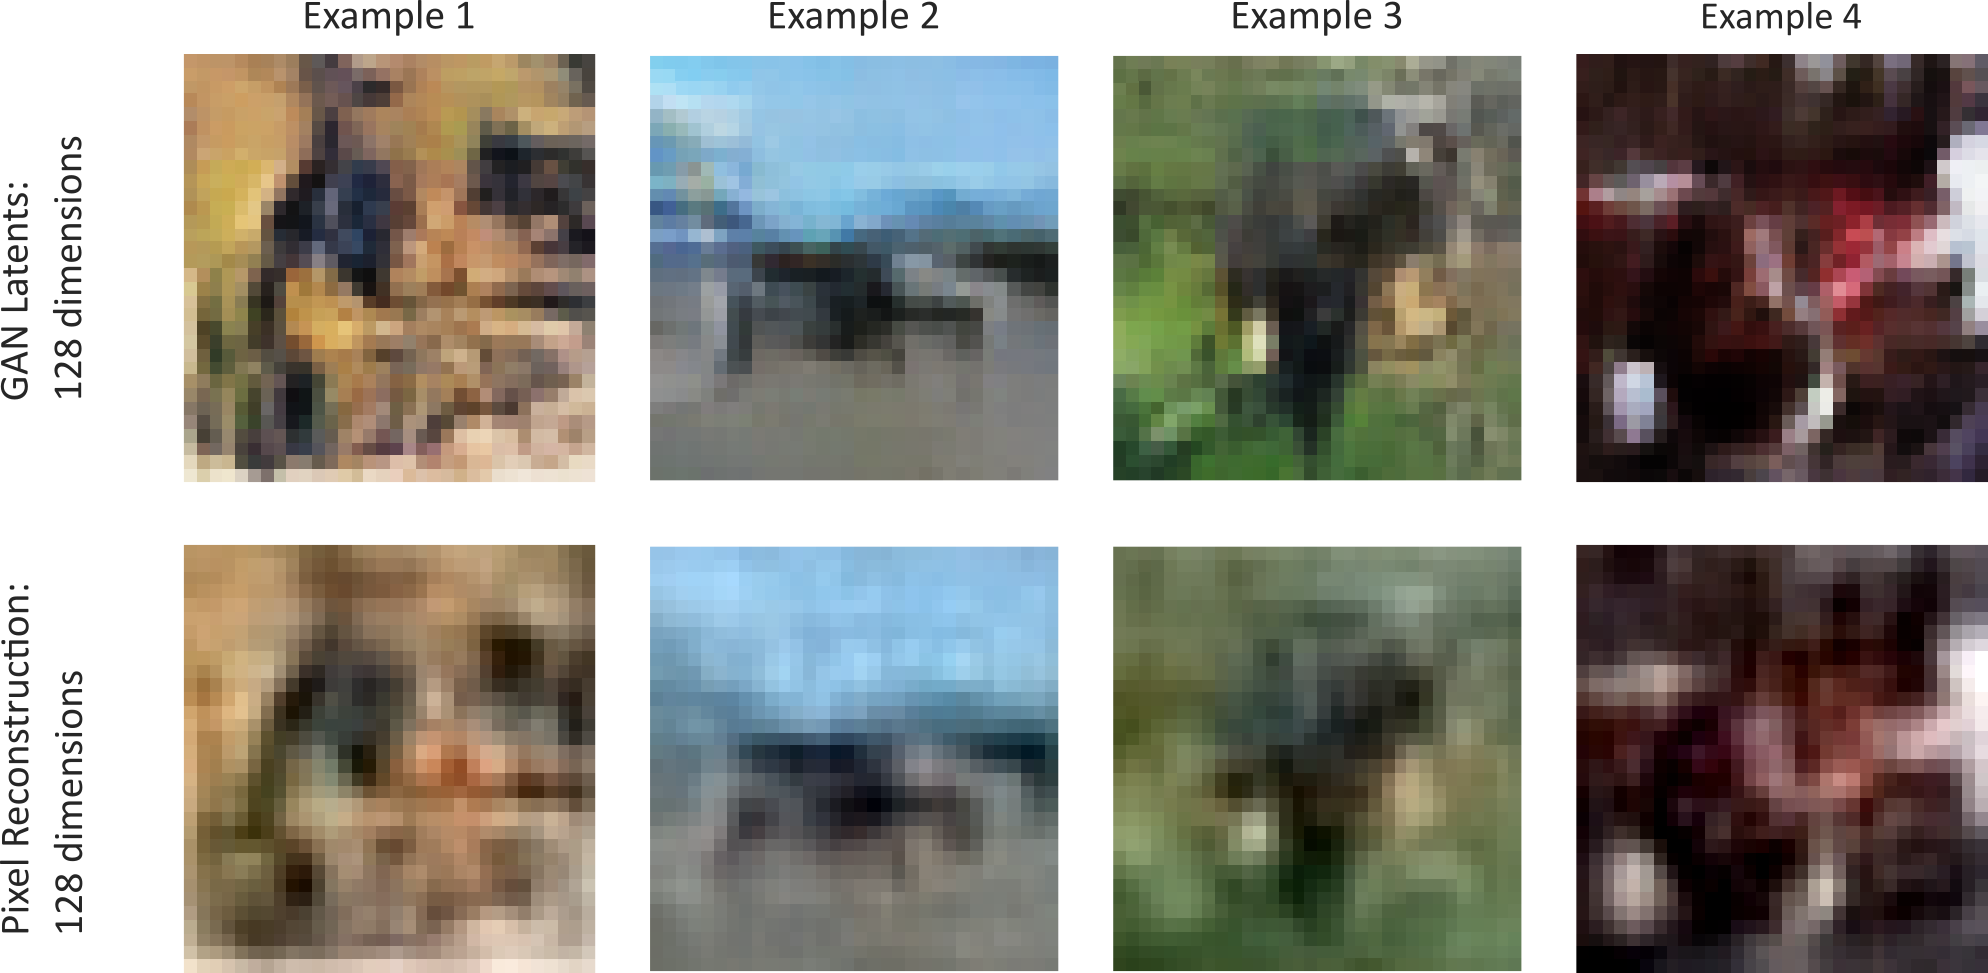
\includegraphics[width=172mm]{exampleImagesWreconstruction.png}
	{\caption{{\it Example GAN Stimuli.} Four example images generated by the 128 GAN latents (top row) and their pixel reconstruction after dimensionality reduction with PCA (bottom row).}
	\label{fig:exampleReconstructions}}
\end{figure}

We first looked at the relationship between stimulus parameters and individual neuron responses. We fit generalized linear models for our 128 GAN latent variables to spike count responses. For each neuron we then also used the actual pixel values shown as predictors for separate models and then compared the AICs in figure \ref{fig:modelAICs}A. As lower AIC indicates a better model, we found that GAN latents are better predictors of neural activity for the majority of neurons (Figure \ref{fig:modelAICs}B).

\begin{figure}
	\centering
	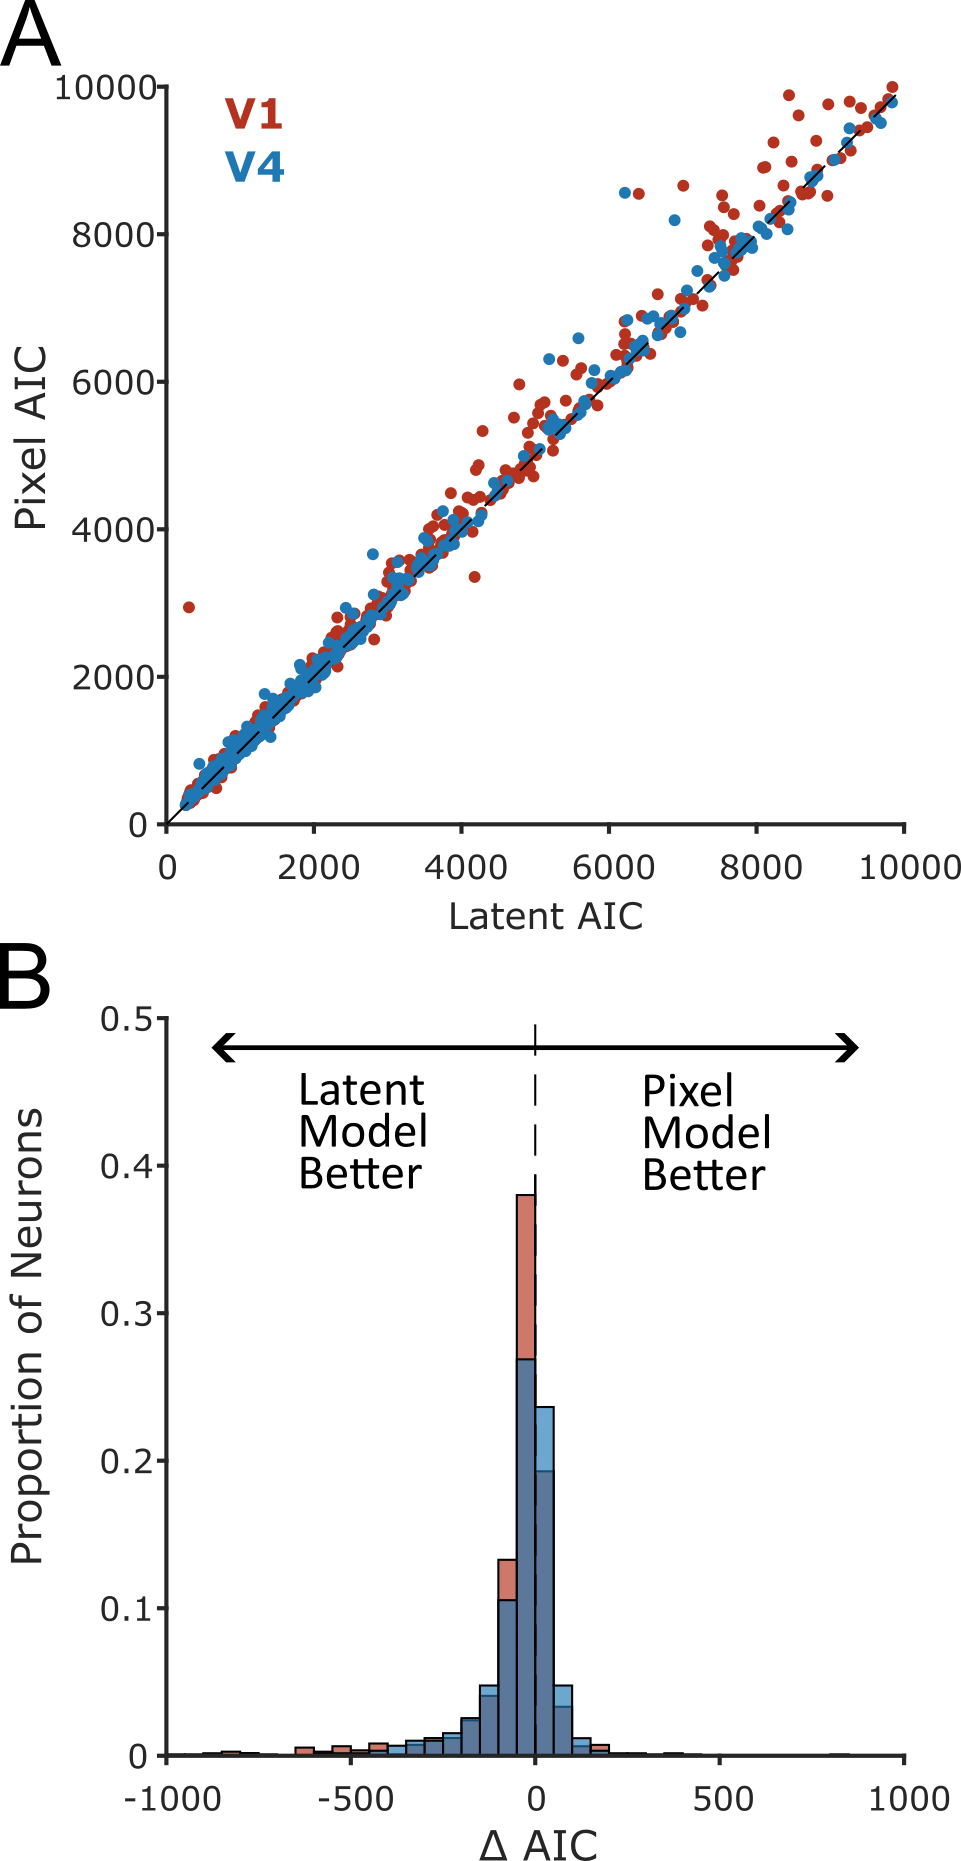
\includegraphics[width=80mm]{LatentVsPixelGLM.png}
	{\caption{{\it Individual neuron model fits} A.) AIC for GLMs using the GAN latents as predictors (x-axis) and the pixel predictors (y-axis) on neuron spike counts. B.) Relative change in AIC across models for individual neurons. Negative values indicate that the GAN latents are better predictors of neural data while positive values indicate that the pixel model was better. The latent model was better on average in both brain regions (V1: $t=-10.26$, $p=1.54 \cdot 10^{-23}$, V4: $t=-6.02$, $p=3.46\cdot 10^{-9}$; t-test).}
	\label{fig:modelAICs}}
\end{figure}

One of the benefits of our approach is the use of high-density electrode recordings afford us population-level analyses of high-dimensional stimuli. The first approach we used to understanding these neural mainfolds is through \gls{cca}. \gls{cca} is a powerful tool in situations where we have high-dimensional predictor variables (latents; Figure \ref{fig:ccaIntuition}A) and high-dimensional response variables (neurons; Figure \ref{fig:ccaIntuition}B). Normally, with a standard basis set, we may find only weak relationships (Figure \ref{fig:ccaIntuition}C). \gls{cca} allows us to take advantage of the dimensionality by rotating and organizing the predictor and response spaces to front-load all linear relationships (Figure \ref{fig:ccaIntuition}D). This demonstrates the principal that while the predictor and response spaces in figure \ref{fig:ccaIntuition} don't appear that related at first glance, a simple change of perspective can clarify much.

\begin{figure}
	\centering
	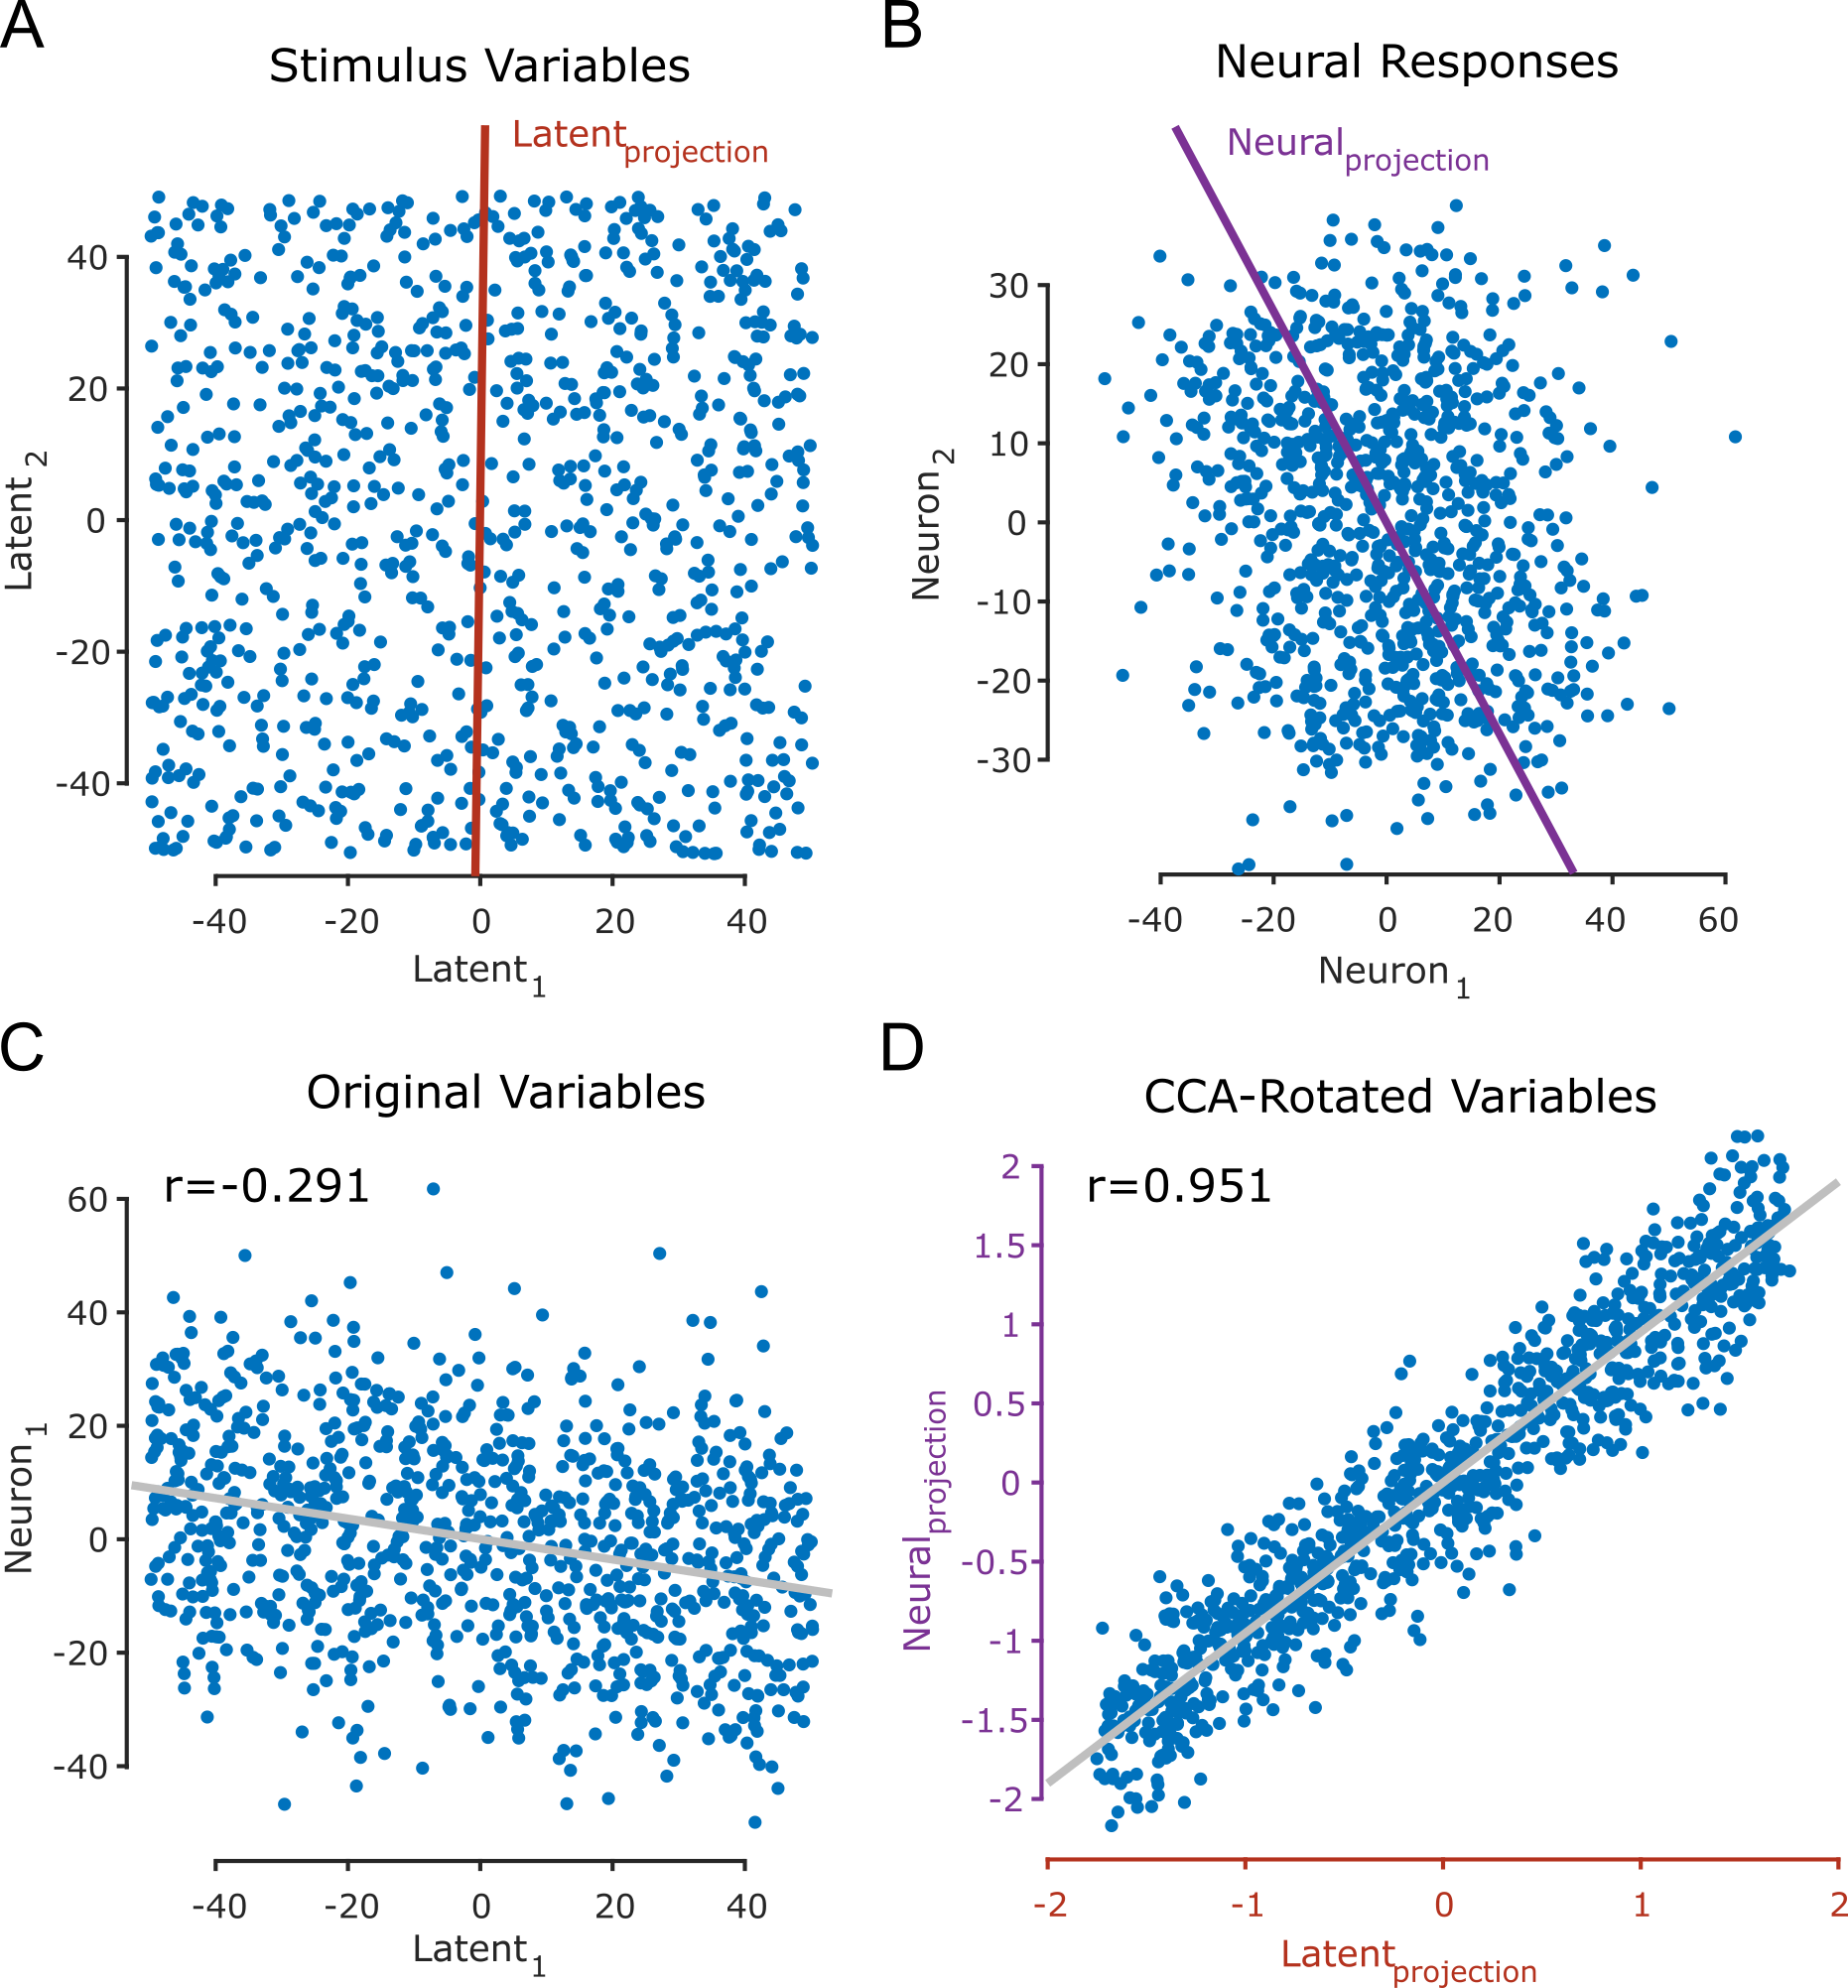
\includegraphics[width=160mm]{CCAintuitionFigure.png}
	{\caption{{\it Canonical Correlations in neural data} A.) Simulated stimulus data where points were randomly selected to span an arbitrary space. The red line indicates the axis chosen by CCA for panel D. B.) Neural state space of stimuli from panel A (each point is paired with a point from A), where each axis is the firing rate of a neuron. Data was centered for visualization purposes as CCA also centers data. The purple line indicates the axis in neural space chosen by CCA for panel D. C.) Original correlation between neuron 1 (panel B) and latent 1 (panel A). D.) First canonical variable pair from the data in panels A and B. The X and Y axes are now linear combinations of the latent and neural dimensions respectively. }
	\label{fig:ccaIntuition}}
\end{figure}

We solved the problem of which stimuli to show using one of three optimization algorithms: \gls{pso}, genetic algorithm, or randomly selected stimuli. We then used \gls{cca} on 6 sessions, one for each algorithm in each brain area, and calculated the correlation between neural activity and GAN latent variables. Directly comparing these values poses a problem though, as \gls{cca} is sensitive to the original dimensionality. So if one session has more or fewer neurons, their correlations wont be comparable. To correct for this we boostrapped \gls{cca} on permuted data within session 100 times and subtracted out what correlations would be expected at chance (Figure \ref{fig:ccaR}). In both V1 and V4, the genetic algorithm outperformed both \gls{pso} and random in finding significantly tuned latent dimensions. Linear stimulus tuning was uncovered even when no optimization was performed, lending credence to the idea that this tuning to GAN latent dimensions is real and not an artifact of optimization.

\begin{figure}
	\centering
	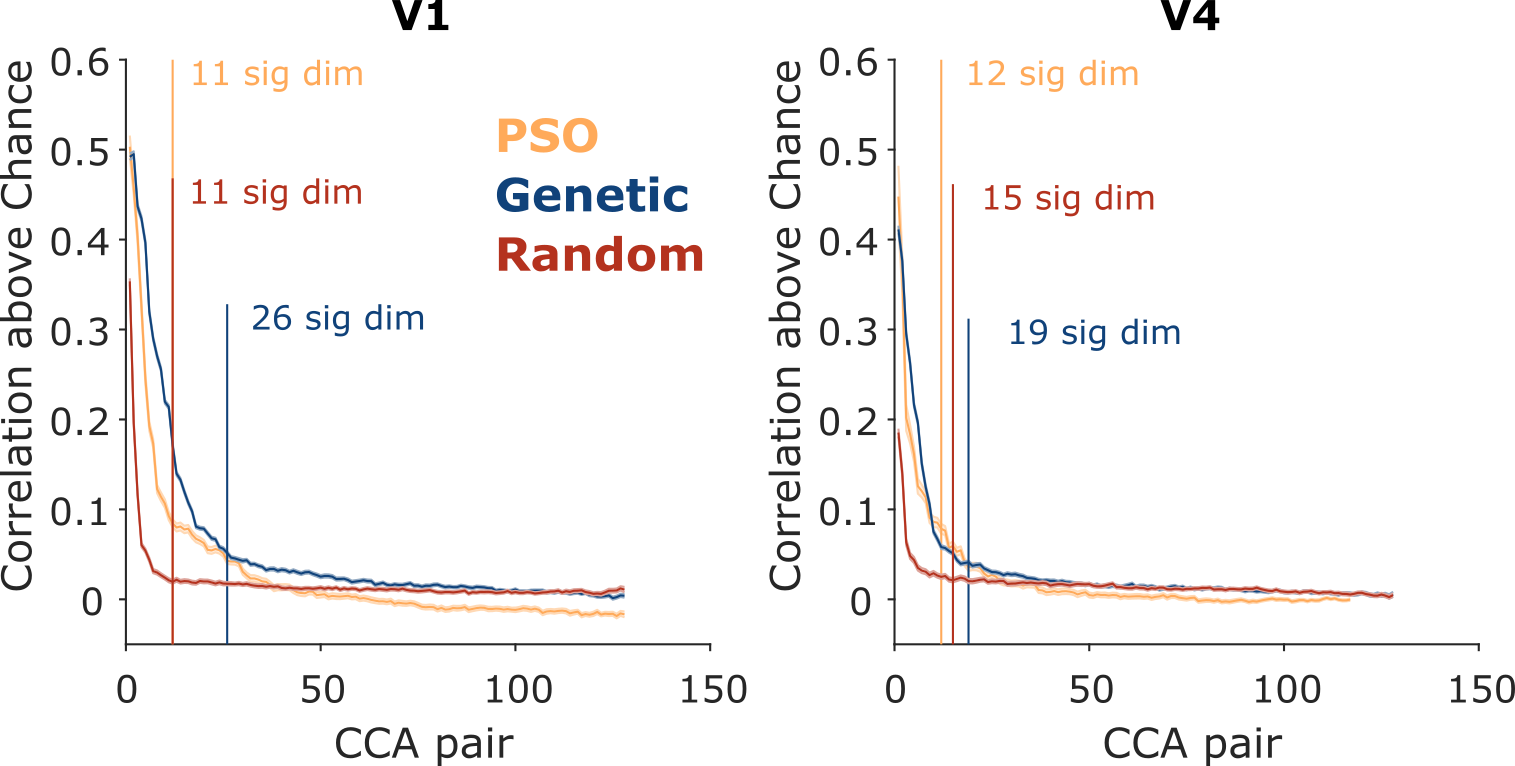
\includegraphics[width=130mm]{CCArValuesByAlgorithm.png}
	{\caption{{\it Baseline-Corrected R values} The baseline-corrected r values for each canonical variable pair across brain region and algorithm. Baseline correction was calculated by subtracting out the distribution of r values calculated from randomly permuting predictors and calculating CCA 100 times. The number of significant CCA pairs was calculated using Rao's approximate F statistic.}
	\label{fig:ccaR}}
\end{figure}

We next wanted to take a closer look at the specific neuron-focused stimulus dimensions that were uncovered in these experiments. In figure \ref{fig:cca1V1}, we show the strongest linear relationships between neurons and \gls{gan} latents across the algorithms. Interestingly, both optimization algorithms found similar ideal dimensions characterized by high contrast dark patches on yellow-green backgrounds (Figure \ref{fig:cca1V1}G\&H). We also see that randomly presenting stimuli results in a much more coarse feature dimension that is largely just light vs dark patches (Figure \ref{fig:cca1V1}I). This is in line with previous studies in V1, and our understanding of simple cells responding best to monochromatic, high-contrast gabors. As for how the algorithm explored the neural manifolds, \gls{pso} transitioned much more smoothly (Figure \ref{fig:cca1V1}D) while the genetic algorithm jumped around more sporadically (Figure \ref{fig:cca1V1}E). Despite the different approaches, it is reassuring to see similar features arise across algorithms that tie in neatly to prior studies in V1.

\begin{figure}
	\centering
	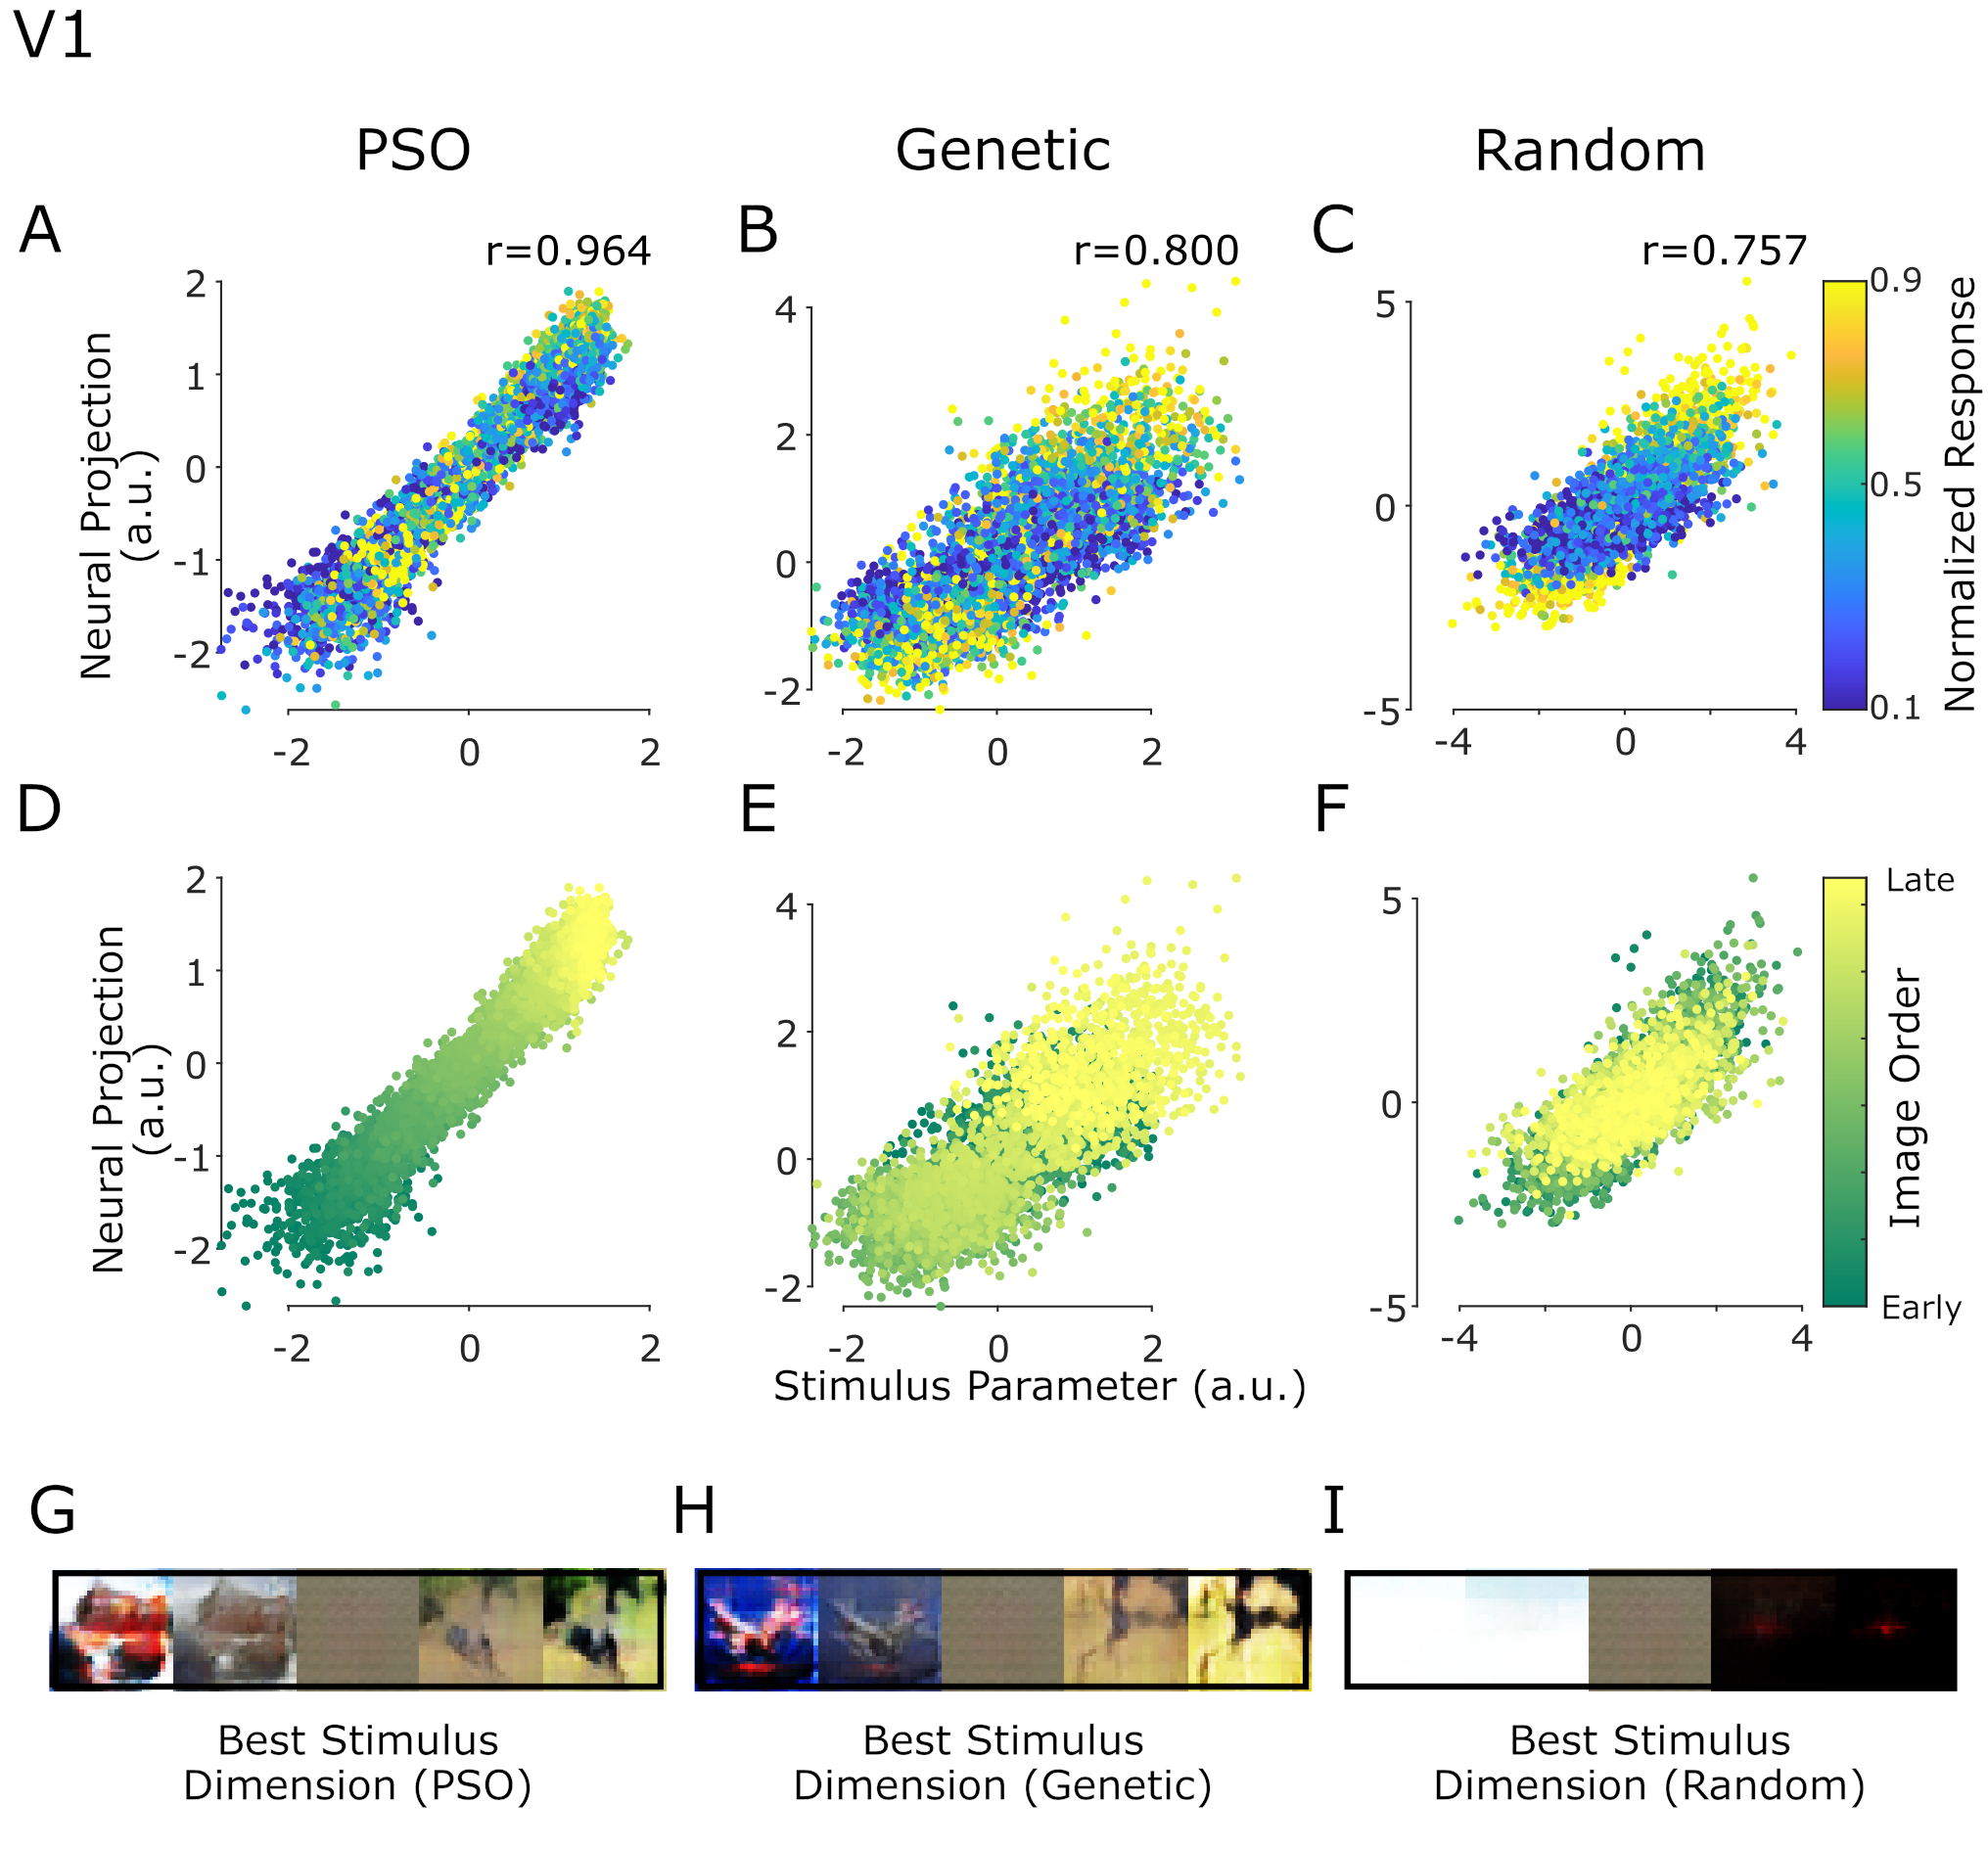
\includegraphics[width=172mm]{CCA1acrossAlgorithmsV1.png}
	{\caption{{\it Linear Relationships in V1} A.) Top CCA pair for a PSO session in V1. Each point is one stimulus and color indicates the normalized $L^2$ norm of the population response vector to that image. B.) Same as panel A for a session optimized with the genetic algorithm. C.) Same as panels A\&B for a session in which no optimization was performed, and instead random images were shown. D-F.) Same as panels A-C except the color now indicates the order of stimuli in the session. G-I.) The GAN latent dimension that CCA found was most linearly related to neural activity for each algorithm. These dimensions correspond to the X-axes in panels A-F.}
	\label{fig:cca1V1}}
\end{figure}

Similar to V1, our experiment found strong linear relationships between the \gls{gan} latent space and neural responses in V4. Again, \gls{pso} and genetic algorithms found starkly similar feature dimensions (Figure \ref{fig:cca1V1}G\&H), while random stimulus presentations found low-contrast global color patches, this time from yellow to blue (Figure \ref{fig:cca1V4}I).

\begin{figure}
	\centering
	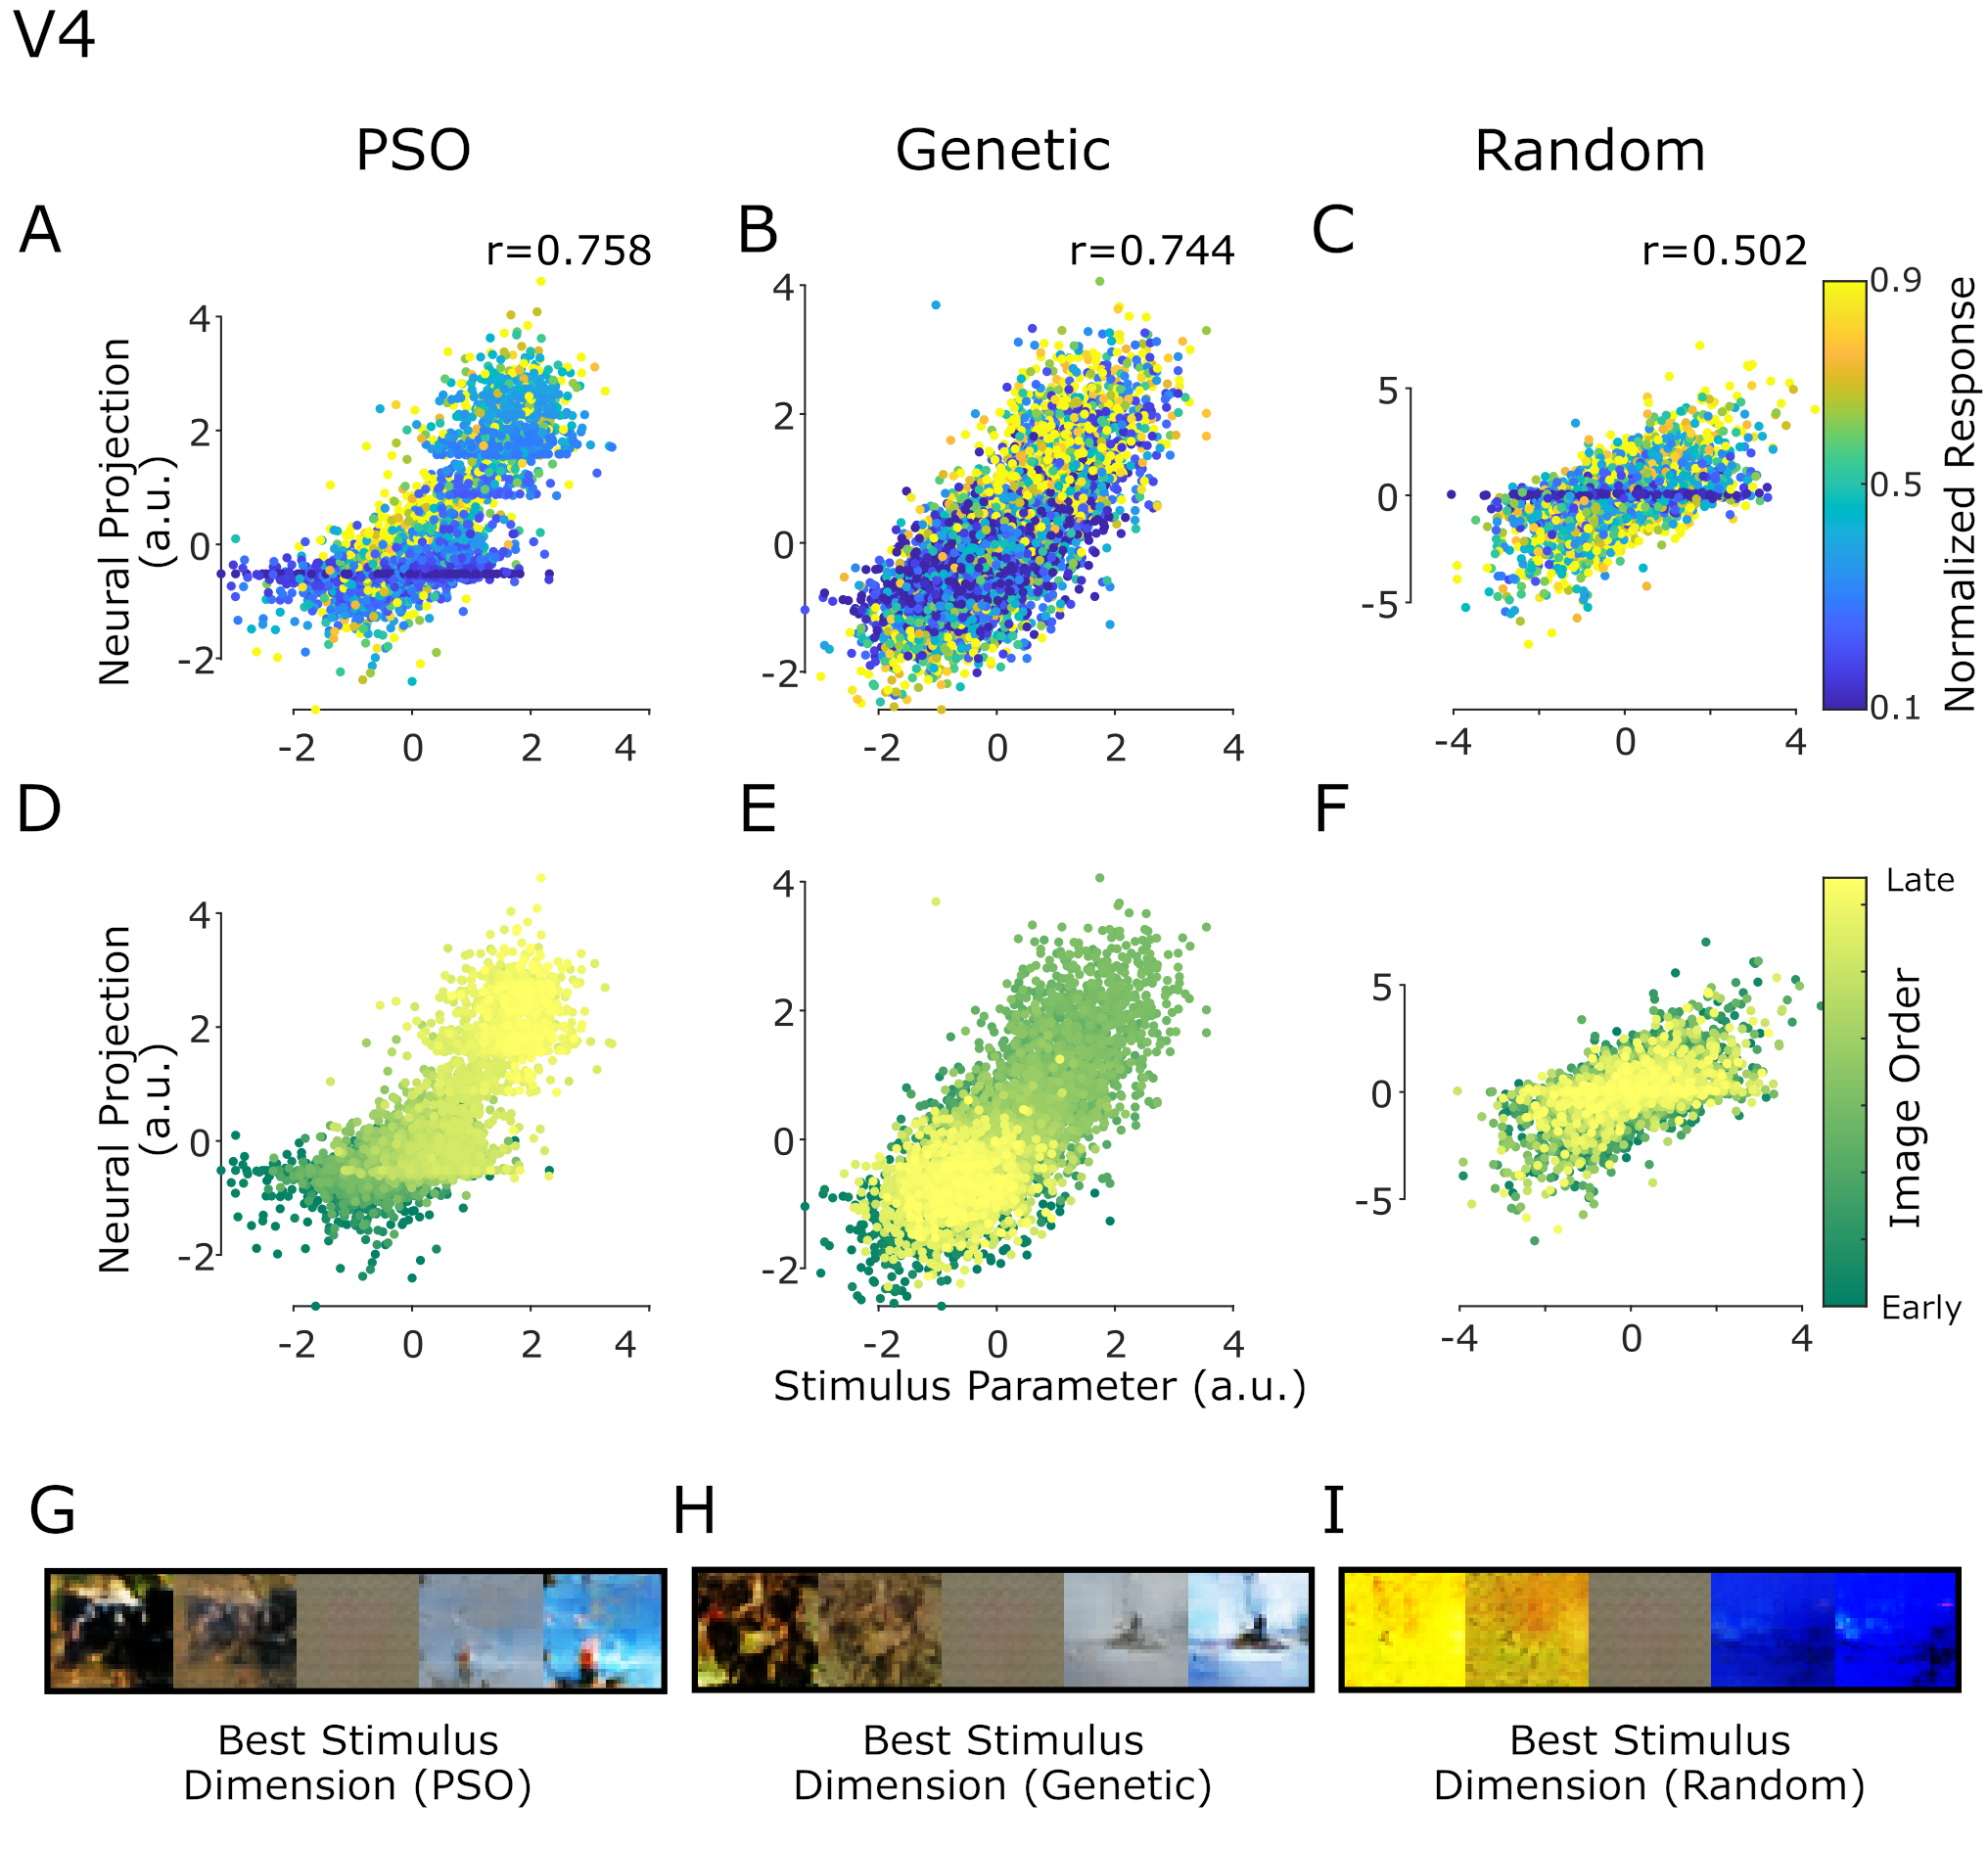
\includegraphics[width=172mm]{CCA1acrossAlgorithmsV4.png}
	{\caption{{\it Linear Relationshipsin V4} A.) Top CCA pair for a PSO session in V4. Each point is one stimulus and color indicates the normalized $L^2$ norm of the population response vector to that image. B.) Same as panel A for a session optimized with the genetic algorithm. C.) Same as panels A\&B for a session in which no optimization was performed, and instead random images were shown. D-F.) Same as panels A-C except the color now indicates the order of stimuli in the session. G-I.) The GAN latent dimension that CCA found was most linearly related to neural activity for each algorithm. These dimensions correspond to the X-axes in panels A-F.}
	\label{fig:cca1V4}}
\end{figure}




\begin{figure}
	\centering
	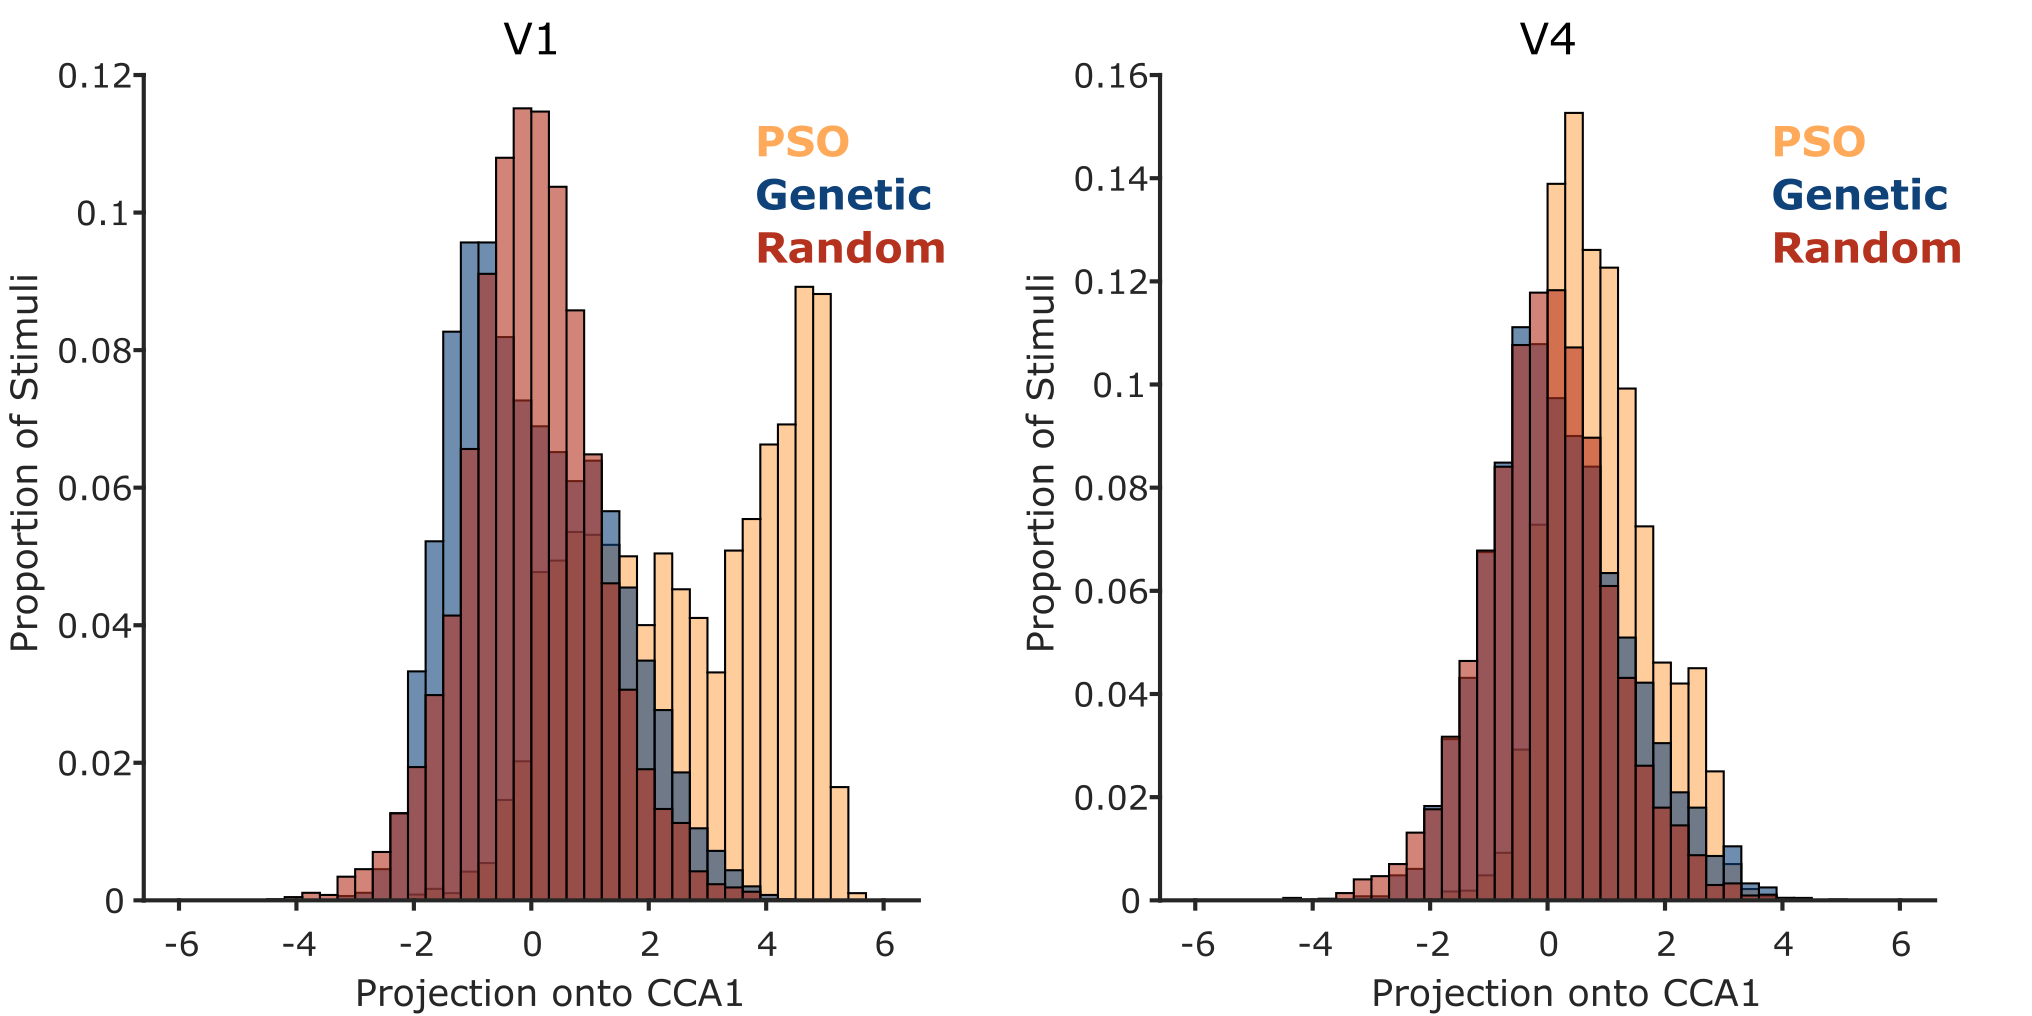
\includegraphics[width=172mm]{cca1ProjectionsCombined.png}
	{\caption{{\it Projections onto CCA1}The value of projections onto Canonical variable pair 1 for each stimulus shown. PSO tends to pick one side of the latent space that it knows has strong optimization evaluations, whereas the genetic algorithm explores more.}
	\label{fig:ccaProjections}}
\end{figure}

 In addition to linear stimulus-response functions, it is well known that mid-level visual areas like V4 demonstrate nonlinear tuning depending on the visual features tested. For example, \cite{Kim2019} found that neurons in V4 combine shape and texture information in ways not directly predictable by the responses to them separately. In order to test the linearity of this stimulus embedding, we decided to use an approach similar to \gls{cca}, \gls{dca}. Instead of maximizing the correlation between pairs of stimulus/response dimensions, \gls{dca} maximizes the distance covariance. One of the drawbacks of pearson correlation is that a value of 0 does not necessarily mean the variables are independent, a drawback that distance correlation does not share. \textbf{In this way, \gls{dca} can be conceptualized as a version of \gls{cca} where both linear and nonlinear relationships are taken into account.} We ran \gls{dca} on the same sessions as \gls{cca} and calculated the distance correlation and significance following \cite{Shen2022}. All three session in both brain areas resulted in significant relationships between the \gls{gan} and neural responses, though to different degrees.
 
\begin{figure}
	\centering
	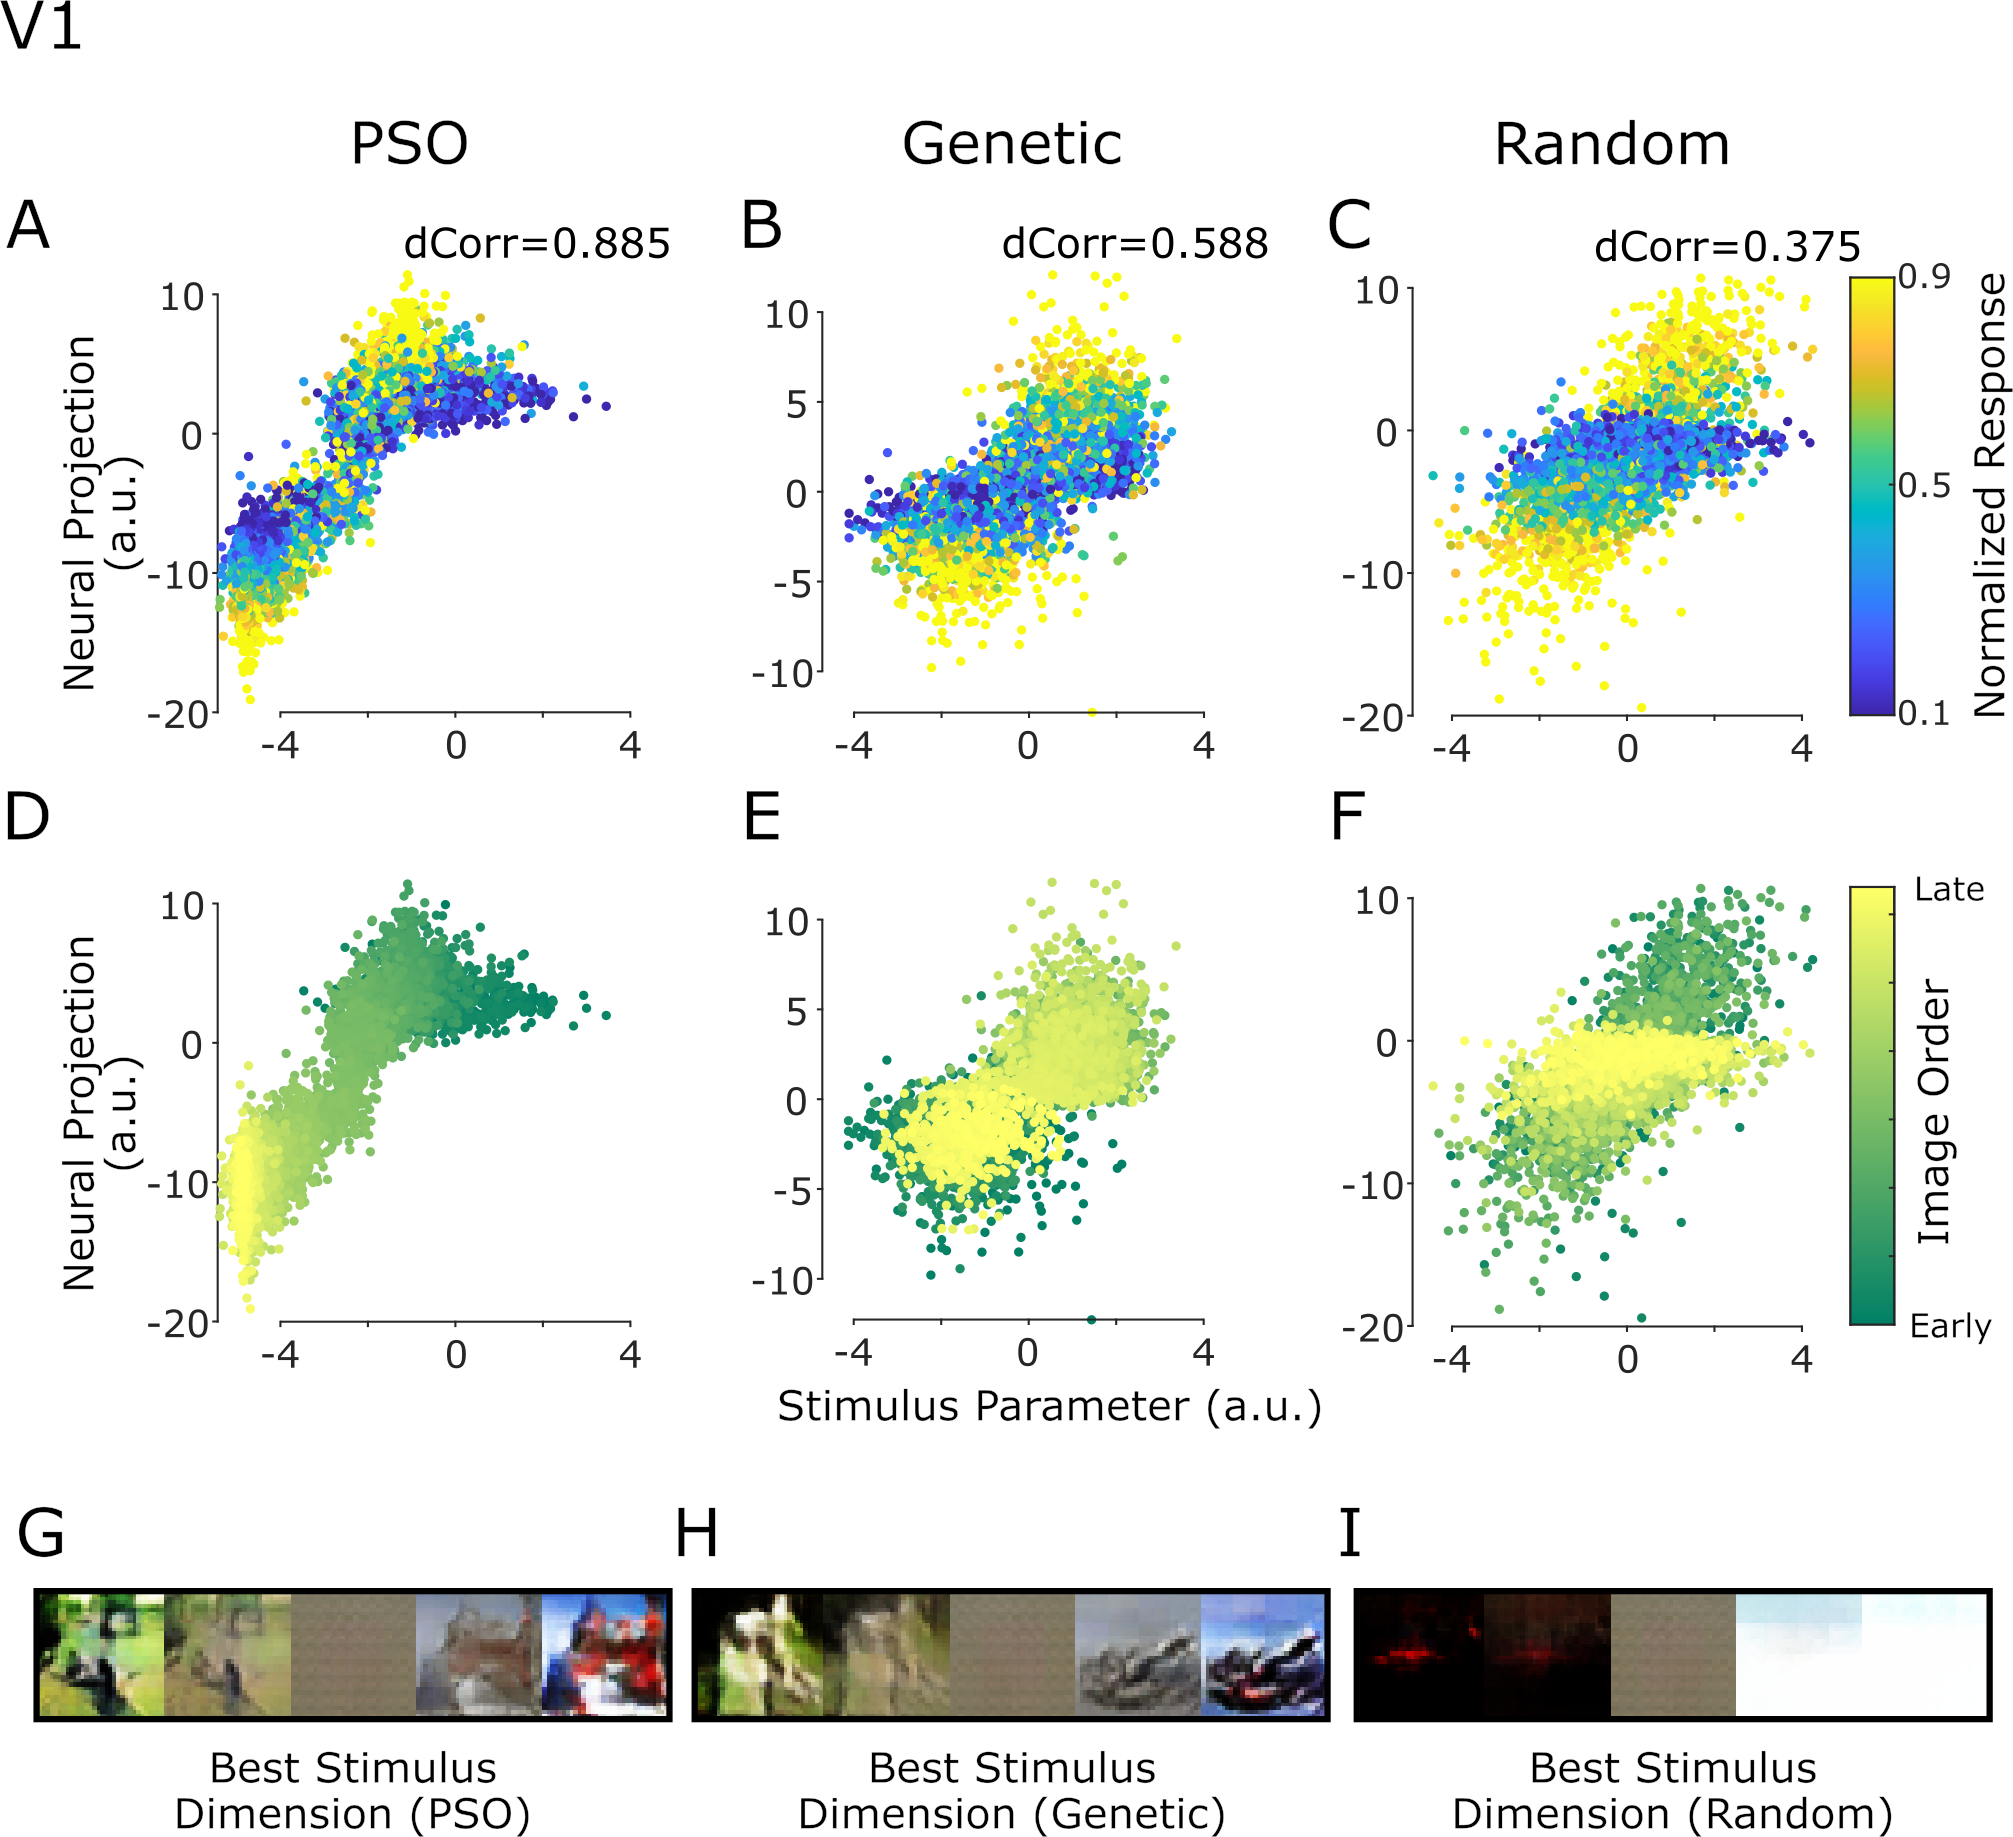
\includegraphics[width=172mm]{DCA1acrossAlgorithmsV1.png}
	{\caption{{\it DCA pair 1 in V1 across Algorithms} A.) Top DCA pair for a PSO session in V4. Each point is one stimulus and color indicates the normalized $L^2$ norm of the population response vector to that image. B.) Same as panel A for a session optimized with the genetic algorithm. C.) Same as panels A\&B for a session in which no optimization was performed, and instead random images were shown. D-F.) Same as panels A-C except the color now indicates the order of stimuli in the session. G-I.) The GAN latent dimension that DCA found was most strongly related to neural activity for each algorithm. These dimensions correspond to the X-axes in panels A-F.}
	\label{fig:dca1V1}}
\end{figure}


\begin{figure}
	\centering
	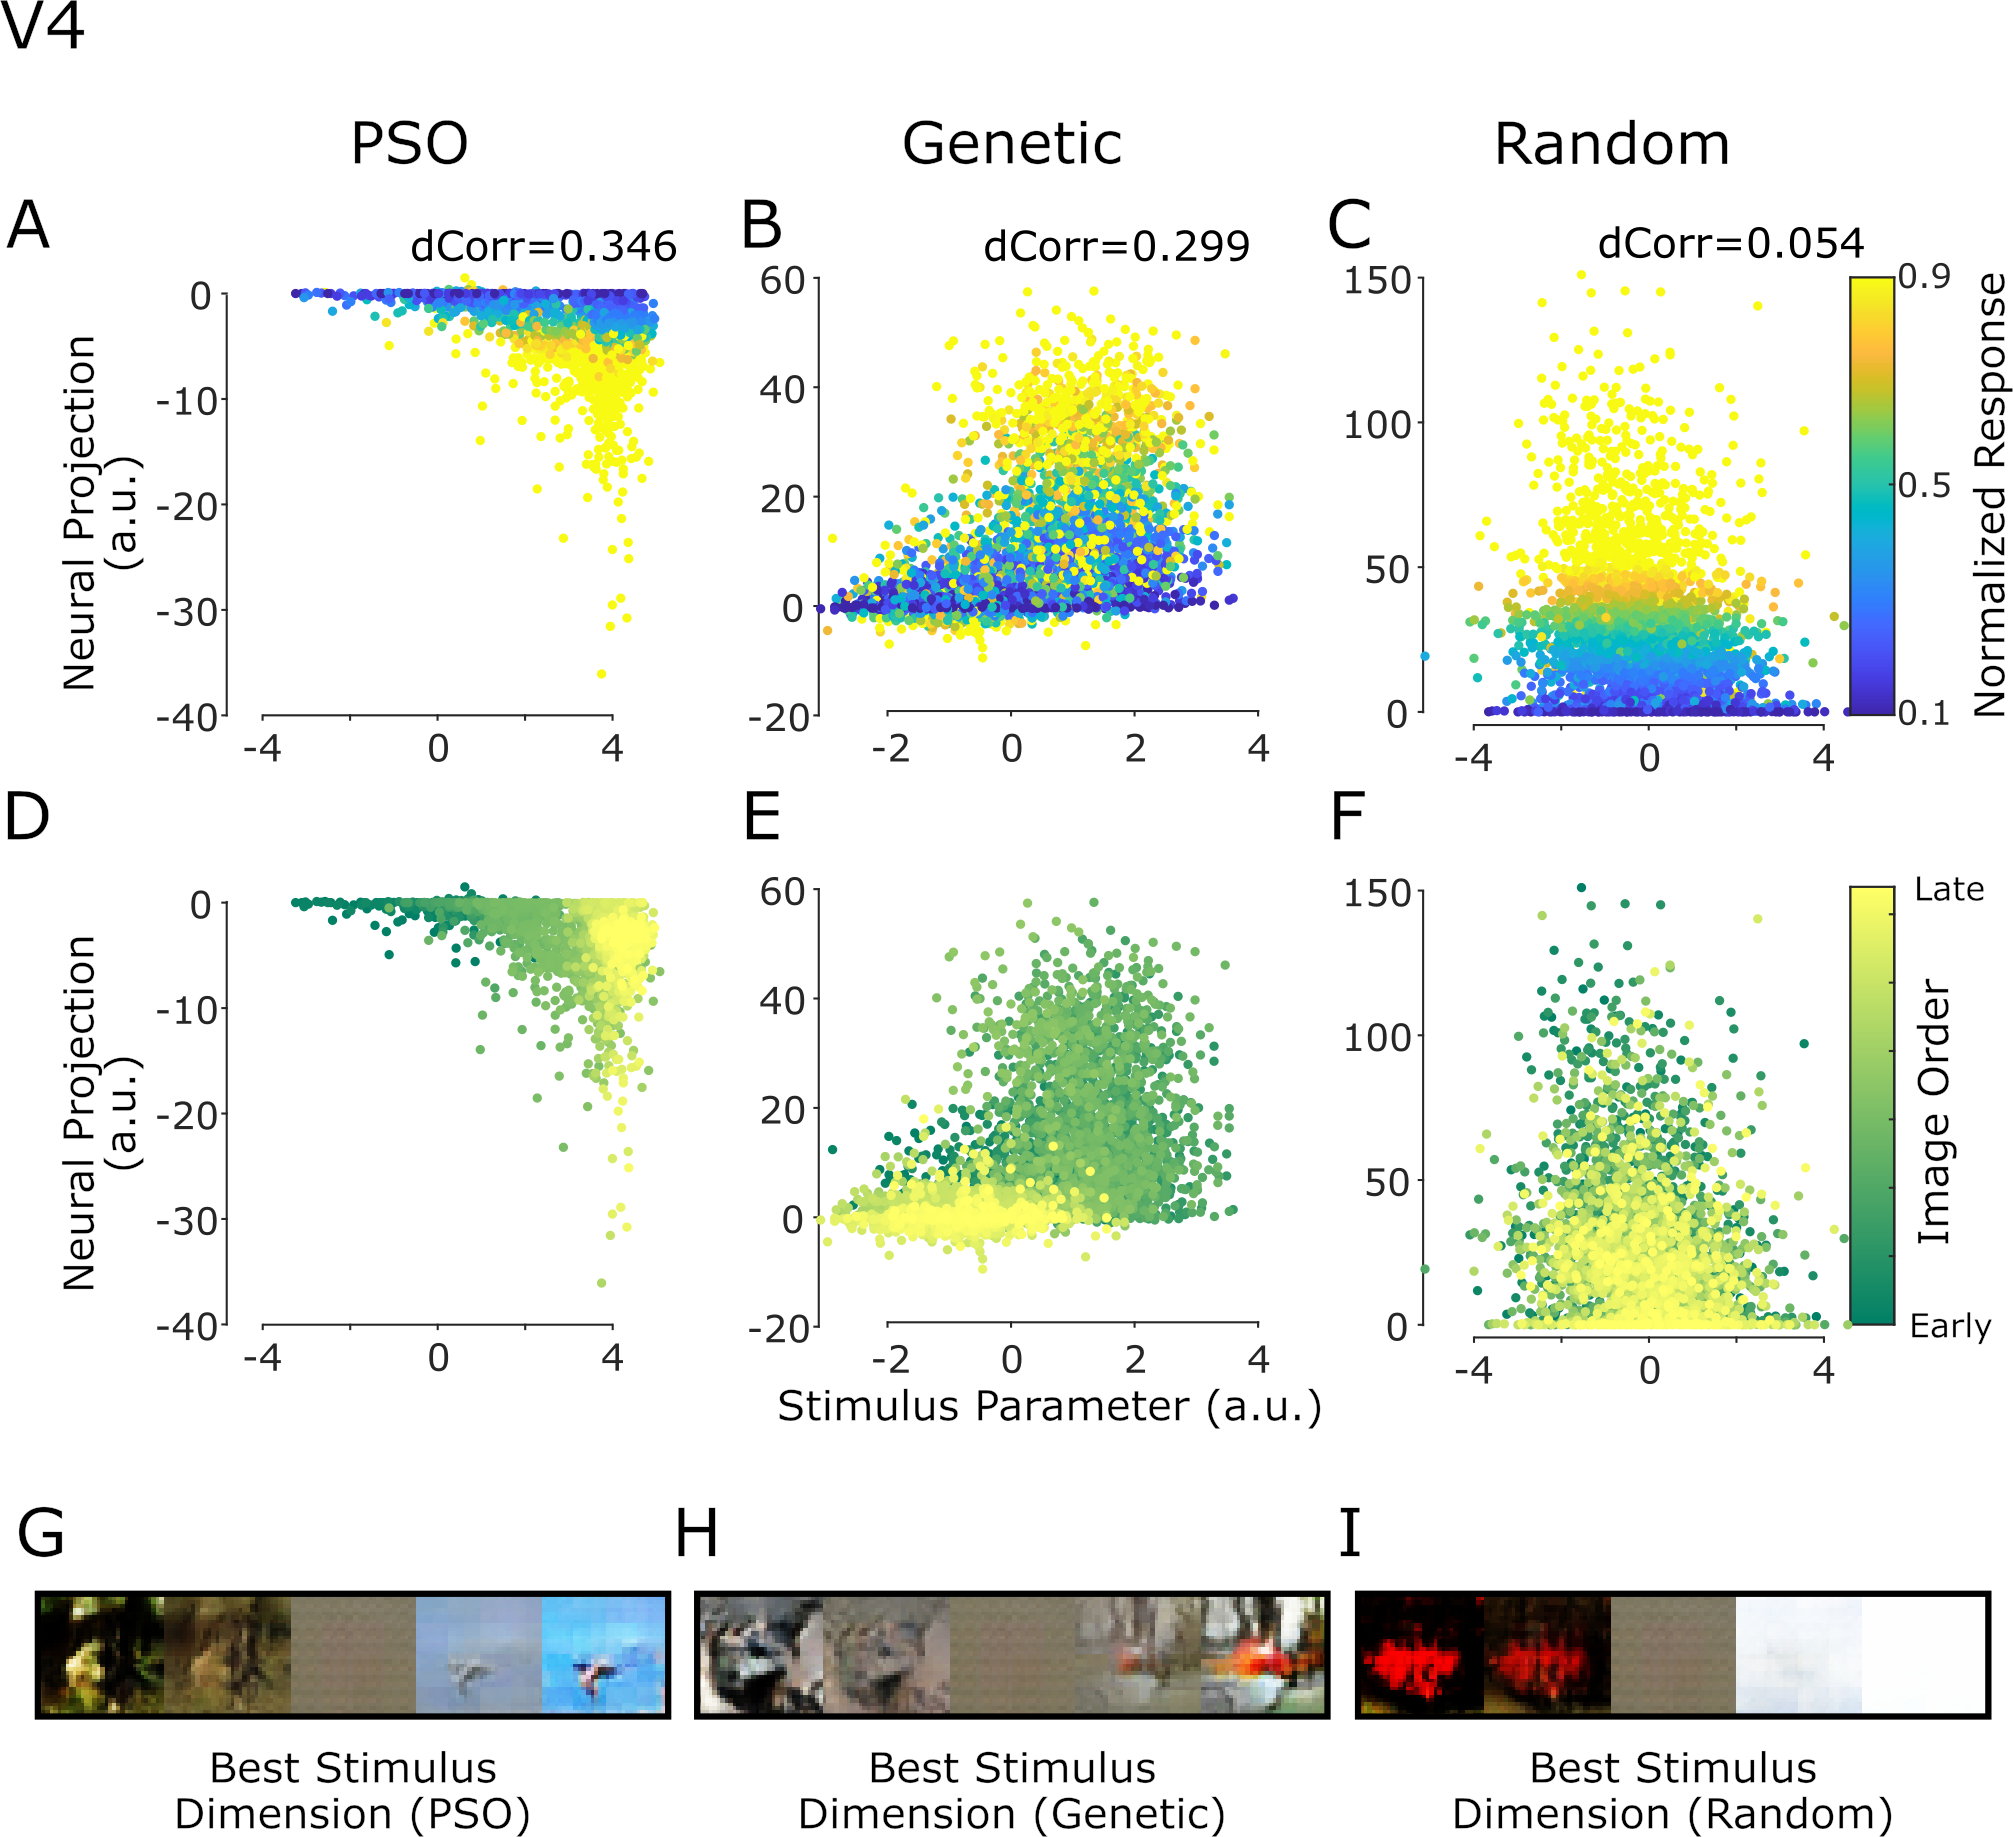
\includegraphics[width=172mm]{DCA1acrossAlgorithmsV4.png}
	{\caption{{\it DCA pair 1 in V4 across Algorithms} A.) Top DCA pair for a PSO session in V4. Each point is one stimulus and color indicates the normalized $L^2$ norm of the population response vector to that image. B.) Same as panel A for a session optimized with the genetic algorithm. C.) Same as panels A\&B for a session in which no optimization was performed, and instead random images were shown. D-F.) Same as panels A-C except the color now indicates the order of stimuli in the session. G-I.) The GAN latent dimension that DCA found was most strongly related to neural activity for each algorithm. These dimensions correspond to the X-axes in panels A-F.}
	\label{fig:dca1V4}}
\end{figure}

Another question we had was how linear the stimulus-response relationship was across brain region. In order to test this we calculated relative linearity (\hyperref[{methods:relativeLinearity}]{Methods}). This metric calculates the distance covariance for the data and the residuals from \gls{cca}, and provides a single number $x \in [-1,1]$ that parses out the contribution of linearity to the distance covariance for each dimension found with \gls{dca}. We did this for both \gls{gan} and pixel predictors in V1 and V4, and found that regardless of algorithm and predictors, V1 maintained consistently linear whereas V4 had a much more nonlinear contribution to the stimulus-response function (Figure \ref{fig:dcaLinearity}).
	
\begin{figure}
	\centering
	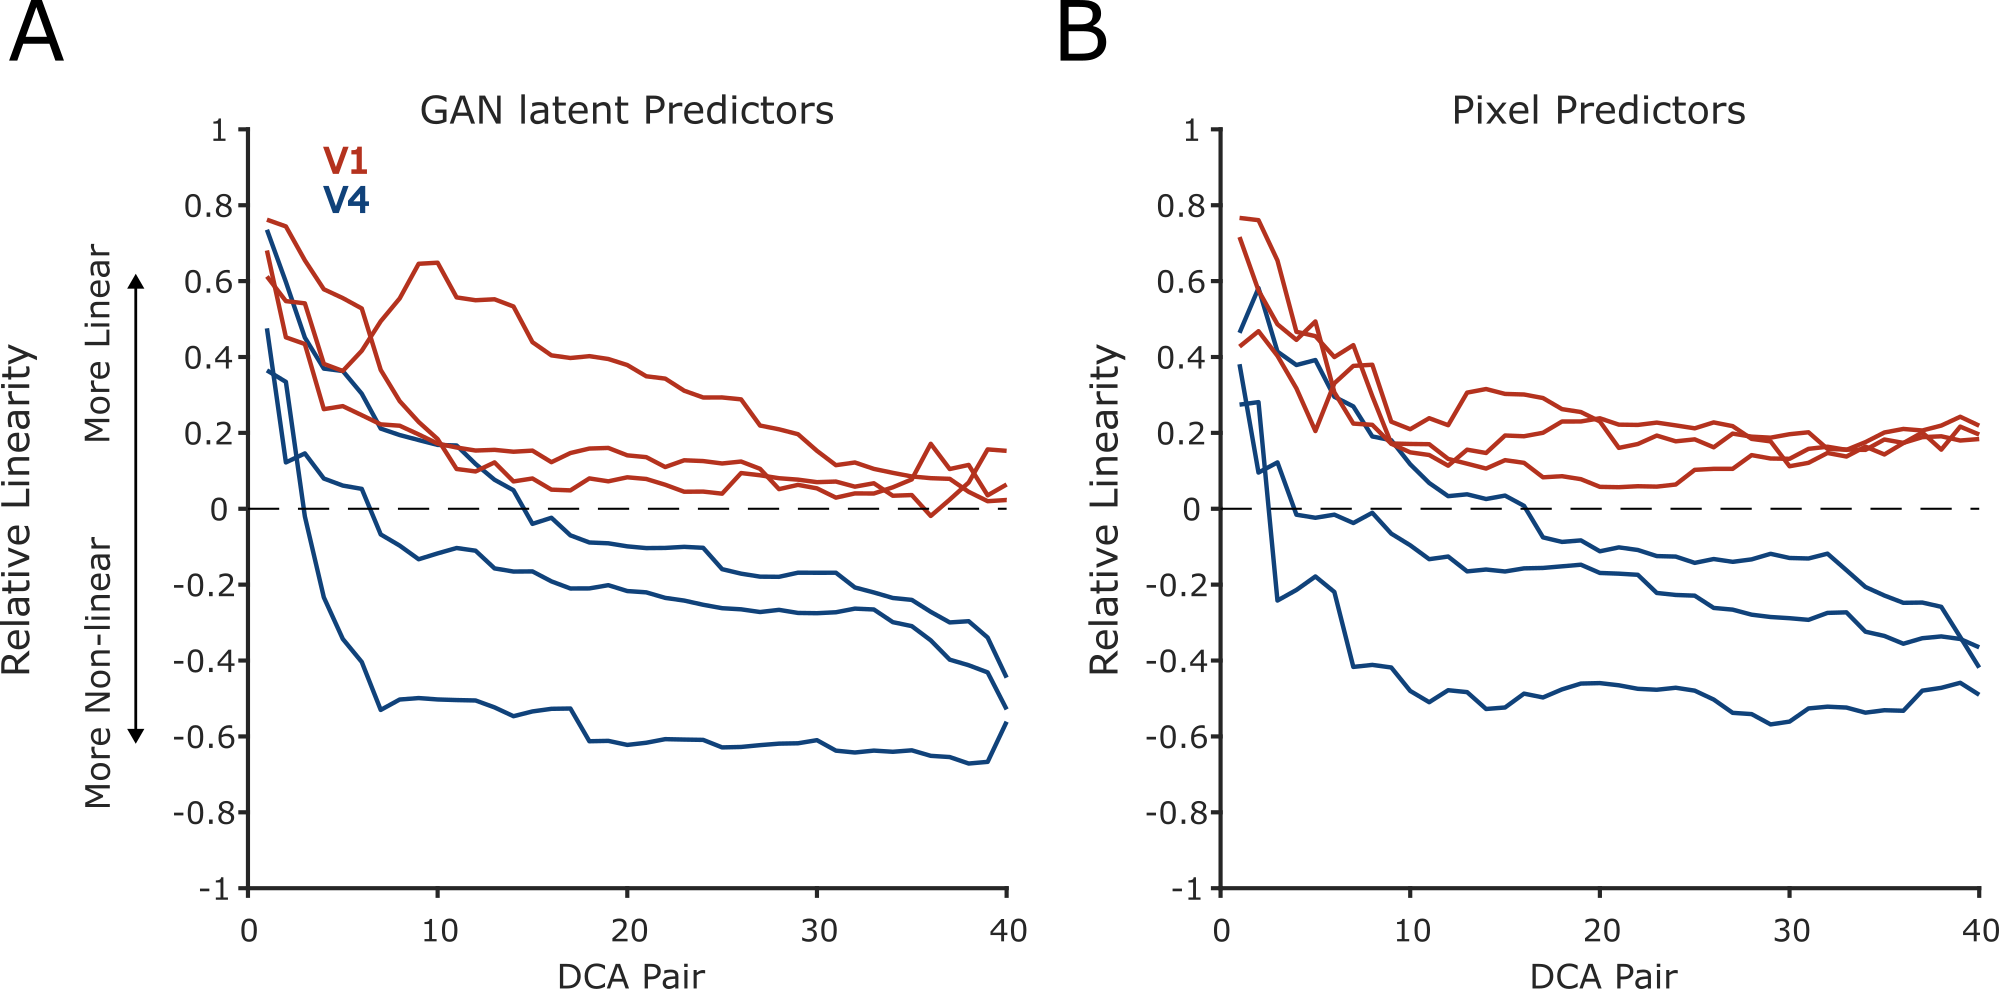
\includegraphics[width=172mm]{DCAresidualDCAbyBrainRegion.png}
	{\caption{{\it Relative Linearity by Brain region} A.) Linearity of neural/stimulus relationships by DCA dimension pairs. Stimulus parameters used were the GAN latent variables. DCA dimensoin pairs are organized by descending distance covariance and relative linearity was calculated as described in \hyperref[{methods:relativeLinearity}]{Methods}. Each line represents one session, and is colored according to brain area. B.) Same as panel A for pixel predictors.}
	\label{fig:dcaLinearity}}
\end{figure}


\section{Discussion}
\glsresetall
In this paper we sought to investigate the relationship between neural population activity and the high-dimensional naturalistic stimulus space generated by a \gls{gan}. Our goal was to develop a pipeline for one-stop-shopping tuning analyses that removed assumptions about brain area, stimulus parameters, and optimization approach. We presented procedurally-generated stimuli to subjects while recording in either V1 or V4, using optimization on the $L^2$ norm of the population response vector to search the neural response manifold. Stimuli were generated using one of three approaches: \gls{pso}, a genetic algorithm, or random stimuli. We found strong linear and nonlinear relationships between the \gls{gan} latent space and neural response space in both V1 and V4, and the \gls{gan} was an even better model for neural activity than the actual pixel values shown.

For the majority of individual neurons in both brain areas, the model fits were significantly better in latent space than pixel space. One issue with this approach is the necessary compression in pixel space to 128 dimensions. We can see from figure \ref{fig:exampleReconstructions} that this compression distorts the image slightly. One may argue that the \gls{gan} is simply a better compression algorithm for the stimuli than \gls{pca} on pixel values, but we believe this wouldn't explain the strong relationships found between the latents and neural data. This is because there is no a-priori reason to believe that the latent dimensions themselves have any meaning to the brain, but we can see from \gls{cca} that even simple linear relationships are significant (Figure \ref{fig:ccaR}).

\gls{cca} is a relatively simple approach that finds a suitable basis set for both predictor (\gls{gan} latents) and response (neurons) variables in which linear relationships are frontloaded. This is analogous to \gls{pca} but instead of maximizing variance in the first few dimensions, it maximizes pearson correlation between the spaces (Figure \ref{fig:ccaIntuition}). We can then look at specifically how many stimulus dimensions are relevant to the neural populations in question. In figure \ref{fig:ccaR} we see that all three algorithms (\gls{pso}, genetic, random) found significant linear relationships between neural activity and \gls{gan} latents, but to various degrees. In both brain areas, the genetic algorithm outperformed \gls{pso} and random stimuli in finding neurally-relevant stimulus dimensions. Taken together with figure \ref{fig:ccaProjections}, we argue this is due to \glspl{pso} tendency to stick to one side of stimulus space that it has determined has large function evaluations whereas the genetic algorithm is free to jump around the space during the recombination and mutation steps. On the other hand, \gls{pso} outperformed the other two approaches when it comes to the strength of the relationships found (Figure \ref{fig:cca1V1}A-C; Figure \ref{fig:cca1V4}A-C). This leads to an important choice for experimenters about the goal of using this technique. If, like most optimization problems, the goal is to find the single best stimulus, \gls{pso} may be the right choice. If however the goal is to explore the neural response manifold, a genetic algorithm may be ideal. In any case, it should not go unmentioned that showing a random set of stimuli with no optimization still provides strong evidence of a relationship between the latent space of a \gls{gan} and neural response space. This shows that any relationships found are not merely artifacts of optimization, but true linear relationships. Another important point to make here, is the similarity between the stimuli found across algorithms (Figure \ref{fig:cca1V1}G-I \& Figure \ref{fig:cca1V4}G-I). It is known that the majority of cells in V1 prefer high contrast light and dark patches, so it is no surprise then that randomly showing naturalistic images pulls out the stimulus dimension in figure \ref{fig:cca1V1}I. The optimization then serves to fill in some of the details around where the contrast edges should be (Figure \ref{fig:cca1V1}G\&H). V4 on the other hand, is more tuned to color (Figure \ref{fig:cca1V4}I) and texture (Figure \ref{fig:cca1V4}G\&H), similar to prior findings in V4 \parencite{Nigam2021, Kim2019}.

An important next step to consider is that the stimulus-response function may not be a linear one \parencite{Prenger2004, Touryan2015}). We sought to determine the degree to which V1 and V4 responded linearly and non-linearly to these complex naturalistic images. In order to do so, we utilized a technique similar to \gls{cca} called \gls{dca} \parencite{Cowley2017}. Instead of maximizing the pearson correlation, \gls{dca} finds new basis sets that maximize the distance covariance. We then calculated distance correlation which unlike Pearson correlation, can directly refer to the degree of variable independence (a distance correlation of 0 indicates independence). Again, both V1 and V4 neurons were significantly related to the latent space of our \gls{gan} (Figures \ref{fig:dca1V1} \& \ref{fig:dca1V4}). As we were interested in the relative contribution of linear and non-linear neural responses, and distance correlation considers both linear and non-linear relationships, we then needed to parse out the linear component. This would allow us to compare within session and brain region, how linear the neural responses were. We again ran \gls{dca}, but this time on the residuals of the \gls{cca} analyses, thus providing a distance correlation for the purely non-linear component. By comparing $dCov_{raw}$ and $dCov_{residual}$ (methods \ref{methods:relativeLinearity}), we can directly compare across sessions and brain regions how linear the neural responses were to these naturalistic images. There are two possibilities for how this analysis could turn out. The first is that because V1 is lower in the hierarchy, it will respond more linearly to both latent and pixel variables than V4. The other hypothesis, is that V1 will be more linearly related to the pixel predictors and more nonlinear to the latents (and vice versa for V4). This may have been the case due to the captured non-linearities within the architecture of the \gls{gan}. Our data supports the former according to figure \ref{fig:dcaLinearity}A. Here we showed that the strongest relationships between latents and neural activity (low \gls{dca} dimensions) in both brain areas were largely linear ($RL>0$). While all stimulus-response relationships were linear in V1, we found many more dimensions with strong non-linear contributions in V4. These trends held true regardless of whether we used the \gls{gan} latent space or pixel space (Figure \ref{fig:dcaLinearity}B). All together, this study demonstrates an important step toward understanding the relationship between high-dimensional stimulus spaces and neural populations in the visual system. 


\section{Conclusion}
\glsresetall
We combined high-density neural recordings in V1 and V4 with techniques pulled from machine learning and artificial intelligence to investigate neural tuning to naturalistic stimuli. We used the latent space of a
\gls{gan} as a stimulus space and searched it using various optimization techniques to maximize the firing rate of our recorded neural population. This lead to confirmation of both prior studies of stimulus tuning in V1/V4 with fewer assumptions, as well as discovering linear and non-linear contributions to neural manifolds. Future work should continue to explore the geometry of neural manifolds in more and more naturalistic settings.

%------------------------------------------------------------------------------------



%------------------------------------------------------------------------------------


 